% !!!!!!!!!!!!!!!!!!!!!!!!!!!!!!!!!!!!!!!!!!!!!!!!!!!!!!!!!!!!!!!!!!!!!!!!!!!!
%                                                                            !
% Adapt this file so that you can use it for your thesis					 !
%                                                                            !
% !!!!!!!!!!!!!!!!!!!!!!!!!!!!!!!!!!!!!!!!!!!!!!!!!!!!!!!!!!!!!!!!!!!!!!!!!!!!


\documentclass{micro-econ-thesis}
\usepackage{graphicx}
\usepackage{setspace}
\usepackage{float}
\usepackage[utf8]{inputenc} % depends on the font encoding that you are using


\usepackage{gensymb}
\usepackage{amsmath}
\usepackage{booktabs}

\usepackage{chngcntr}
\usepackage{caption}

\counterwithout{table}{section}


% For formatting of your bibliography, please use the following package with options 
\usepackage[style=authoryear-icomp, maxcitenames=1, minbibnames = 3, maxbibnames=5, backend=biber, uniquelist=true ]{biblatex}

\addbibresource{bibliography.bib} % add a bib-reference file

\AtEveryBibitem{\clearfield{day}}



\begin{document}
% ----------------------------------------------------------------------------
% Details for the titlepage
% ----------------------------------------------------------------------------
\thesisTitle{Development of Analysis Techniques for Dynamic Magnetic Resonance Imaging of the Knee}
\thesisType{Master Thesis} % 'Master Thesis' or 'Seminar Paper'
\thesisAuthor{Aayush Nepal}
\thesisMail{aayush.nepal@uni-jena.de}
\thesisGrade{Master of Science in Medical Photonics} % leave empty for seminar papers
\thesisTutora{Prof. Dr. rer. nat. med. habil. Jürgen Reichenbach}
\thesisTutorb{Dr. rer. nat. Martin Krämer}
\thesisMatrikel{198683}
%\thesisAddress{}
\thesisDate{\today}
% In case of external supervisor
\thesisCompany{}

% Print titlepage
\thesisMakeTitle

% ----------------------------------------------------------------------------
% Abstract
% ----------------------------------------------------------------------------
\cleardoublepage
\pagenumbering{roman}
\pagestyle{plain}
%\thispagestyle{empty}
\subsection*{Abstract}

The knee joint, a critical component of human movement, frequently endures mechanical loads that can lead to degenerative conditions such as osteoarthritis (OA). OA, prevalent globally and particularly affecting the knee, requires early diagnosis for effective intervention. Magnetic resonance imaging (MRI) has proven effective in detecting soft tissue changes, but traditional MRI studies often miss early-stage OA indicators as traditional static MRI measurements are conducted under non-weight-bearing conditions, unlike the actual physiological state during daily activities.

This thesis leverages recent advancements in MRI technology to analyze the knee joint under mechanical loading, using high-resolution CINE MRI imaging. This approach enables the investigation of dynamic interactions between the femur and tibia during flexion-extension cycles, providing detailed(potential) insights into knee mechanics. A major challenge in this process is the accurate segmentation of anatomical structures, across multiple time frames, critical for reliable biomechanical measurements. To address this, a semi-automated segmentation pipeline was developed, streamlining the process and improving consistency across sequential images.

Following segmentation, this thesis quantified biomechanical parameters, such as the angle between the long axes of the femur and tibia and the distance between anatomical landmarks, under various loading conditions. The results showed significant variations in distance measurements during the early phase of flexion, highlighting the knee's sensitivity to external loading. However, no significant differences were found in the angular measurements, suggesting stability in bone alignment under load.

This research demonstrates the potential of semi-automated segmentation for efficient and precise analysis of dynamic knee MRI scans, offering potential advantages for clinical and research applications. Despite the promising findings, the study's reliance on single 2D slices limits the comprehensive assessment of knee kinematics. Future work should extend this methodology to 3D analyses and explore its application to patellofemoral kinematics, providing a more holistic understanding of knee mechanics.

In conclusion, this thesis presents a robust method for analyzing knee joint biomechanics using advanced MRI techniques, paving the way for enhanced diagnostic and research capabilities in orthopedics.

\clearpage
\subsection*{Acknowledgements}


% ----------------------------------------------------------------------------
% Table of contents
% ----------------------------------------------------------------------------
\cleardoublepage
%\thispagestyle{empty}
\tableofcontents

% ----------------------------------------------------------------------------
% List of figures/tables
% ----------------------------------------------------------------------------
\cleardoublepage
\phantomsection
\addcontentsline{toc}{section}{List of Figures}
\listoffigures
% --------------------------
\cleardoublepage
\phantomsection
\addcontentsline{toc}{section}{List of Tables}
\listoftables
% --------------------------

\cleardoublepage
\phantomsection
\addcontentsline{toc}{section}{List of Acronyms}
\section*{List of Acronyms}
\begin{tabular}{@{}ll}
ADMM & Alternating Direction Method of Multipliers \\
BMI & Body Mass Index \\
Cov & Covariance matrix \\
FFT & Fast Fourier Transform \\ 
FLASH & Fast Low Angle Shot \\
FID & Free Induction Decay \\
FoV & Field of View \\
GRE & Gradient Echo \\
MRI & Magnetic Resonance Imaging \\
OA & Osteoarthritis\\
PCA & Principal Component Analysis \\
SEM & Standard Error of the Mean \\
SHM & Screw Home Mechanism \\
TE & Time to Echo \\
TGV & Total Generalized Variation \\
TR & Repetition Time 

\end{tabular}

% --------------------------

% ----------------------------------------------------------------------------
% Contents
% ----------------------------------------------------------------------------
\cleardoublepage
\pagestyle{headings}
\pagenumbering{arabic}
\setcounter{page}{1}
% Contents
\onehalfspacing % for linespacing 1.5, you can turn it off with \singlespacing, e.g. for quotes or tables with multiline cells

\section{Introduction}

The knee joint, a crucial structure in human movement, consists of various tissues with distinct structural and mechanical properties, including articular cartilage and meniscus. These components are regularly subjected to compressive mechanical loads, making them susceptible to degenerative conditions such as osteoarthritis (OA). OA affects a significant portion of the global population and the knee joint is among its common targets, leading to functional impairments and increased healthcare costs \parencite{WHO}. A comprehensive survey across 15 European countries and Israel found that knee pain was the third most commonly reported type of chronic pain, underscoring the significant public health concern it represents \parencite{breivik_survey_2006}. Furthermore, OA was identified as the most common cause of this pain. This situation has not improved over time. In Germany, for instance, a recent retrospective study found that the number of patients with OA is steadily rising \parencite{obermuller_epidemiology_2024}. As society ages, the prevalence and impact of OA are expected to rise, posing significant public health challenges \parencite{yelin_burden_2016}. Knee-related issues are prevalent and impactful due to the inherent complexity of the knee joint itself. As a hub of various anatomical structures working in unison, the knee supports a range of movements and bears significant loads, making it susceptible to a variety of injuries and conditions. Early diagnosis of OA is crucial for timely intervention, and understanding the anatomy of the knee is the first step in tackling this problem. Magnetic resonance imaging (MRI) has emerged as a promising non-invasive technique for early diagnosis of OA due to its excellent soft tissue contrast and high spatial resolution \parencite{kijowski_osteoarthritis_2020}. 

Traditionally, MRI studies aimed at assessing the structure and function of the knee joint have been performed with the joint at rest or in non-weight-bearing conditions, which, however, do not accurately reflect the physiological state of the knee during daily activities \parencite{blankevoort_envelope_1988}. For instance, research has shown that bone marrow lesions, which are associated with osteoarthritis progression, are significantly related to mechanical loading during activities like walking, highlighting the limitations of non-weight-bearing MRIs in detecting early-stage OA \parencite{bennell_bone_2010}. Additionally, dynamic MRI studies have demonstrated that knee kinematics during continuous movement reveal significant differences compared to static positions, providing crucial information that static scans may miss \parencite{dentremont_dynamicbased_2013}.

Recent advancements in MRI technology have enabled the study of knee joints under mechanical loading conditions, better mimicking the actual physiological environment by allowing both controlled application of loads and dynamic movement during imaging \autocites{conconi_-vivo_2023}{jogi_device_2022}. MRI-compatible loading devices facilitate the investigation of how tissues deform and how their morphology changes in response to stress and movement.  Various MRI measures, including tissue deformation from magnitude images, phase information, and quantitative MRI, have been employed to assess these changes. 

Building on these recent advancements in MRI technology, this thesis utilizes high-resolution dynamic MRI to develop a method for analyzing the relative movements between the femur and tibia during flexion-extension cycles under various loading conditions.  This method is then applied to track specific kinematic parameters at various points in the movement cycles, providing a basis for validating the method and conducting detailed biomechanical analyses.

To achieve reliable kinematic analyses, the initial step involves accurately segmenting key anatomical structures from the dynamic MRI sequences. This segmentation is crucial, as it significantly influences the reliability of biomechanical measurements derived from the MRI data. Traditionally, segmentation of musculoskeletal tissues has been performed manually in which a user delineates the boundaries of each joint structure on each MR image slice that is extremely time-consuming with its efficiency and repeatability influenced by the level of user expertise \parencite{mcwalter_use_2005}. This problem is exacerbated when dealing with multiple frames in a dynamic sequence. On the other hand, modern techniques like Convolutional Neural Networks and U-Nets are being widely used to automate the segmentation process \parencite{liu_deep_2018}. Unfortunately, these methods typically require large annotated datasets for training, which are not available for the dynamic knee imaging performed in this project. To address these issues, this thesis proposes the development of a semi-automated pipeline to segment the tibia and femur from the dynamic MRI data, specifically from single-slice 2D images in sagittal view captured throughout the knee's motion cycle under both loaded and unloaded conditions. This new methodology aims to streamline the segmentation process, reducing the time and effort involved across sequential images.

Following the successful segmentation of the bones, the subsequent analysis involves quantifying two distinct biomechanical parameters: the angle between the long axes of the tibia and femur segments and the distance between specific anatomical landmarks on these bones. These parameters were chosen because they naturally capture the relative motion and spatial relationships between the femur and tibia, which are essential for understanding knee joint mechanics. The purpose of this quantification is to investigate how these parameters change throughout the motion cycle and how they vary under loaded and unloaded conditions. Conducting this study on healthy volunteers aims to establish normative trends that can serve as benchmarks for future comparisons with patient data, potentially aiding in the assessment of knee joint stability and functionality. 

\section{Fundamentals}
\label{sec:intro}


\subsection{The Knee Joint }

The knee joint is the largest and the most superficial synovial joint in the body \parencite{dalley_moores_2023}. The anatomy of the knee joint includes several important structures such as bones, cartilage, and ligaments. These components work together to provide stability and flexibility to the joint. Figure \ref{fig:kniearthrosekniegelenk-anatomieenjpg} illustrates the anatomy of the right knee joint, highlighting these key structures.
\begin{figure}[H]
	\centering
	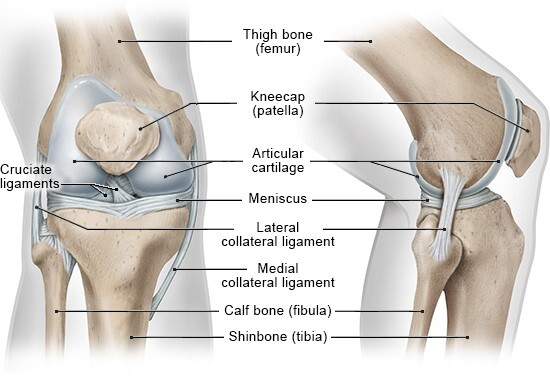
\includegraphics[width=0.7\linewidth]{kniearthrose_kniegelenk-anatomie_enjpg}
	\caption{Anatomy of the right knee joint showing bones, cartilage, and ligaments. Left: front view; Right: side view. Key structures include the femur (thigh bone), tibia (shinbone), fibula (calf bone), patella (kneecap), articular cartilage, meniscus, and various ligaments such as the cruciate ligaments, lateral collateral ligament, and medial collateral ligament. \parencite{informedhealth2021}}
	\label{fig:kniearthrosekniegelenk-anatomieenjpg}
\end{figure}

 
It consists of three compartments that form a dynamic, specialized hinge joint \parencite[p.1395]{standring_grays_2021}. These compartments are the medial compartment, the lateral compartment, and the patellofemoral compartment.
Each compartment contains primary articulations that contribute to the joint's biomechanical performance. Specifically, the knee comprises two femorotibial articulations—one in the medial compartment and one in the lateral compartment (see Figure \ref{fig:rightkneeplate519})—and one femoropatellar articulation in the patellofemoral compartment (see Figure \ref{fig:patellarsurface}).  These articulations, illustrated in  are defined by their complexity and incongruence. 
 
\begin{figure}[H]
	\centering
	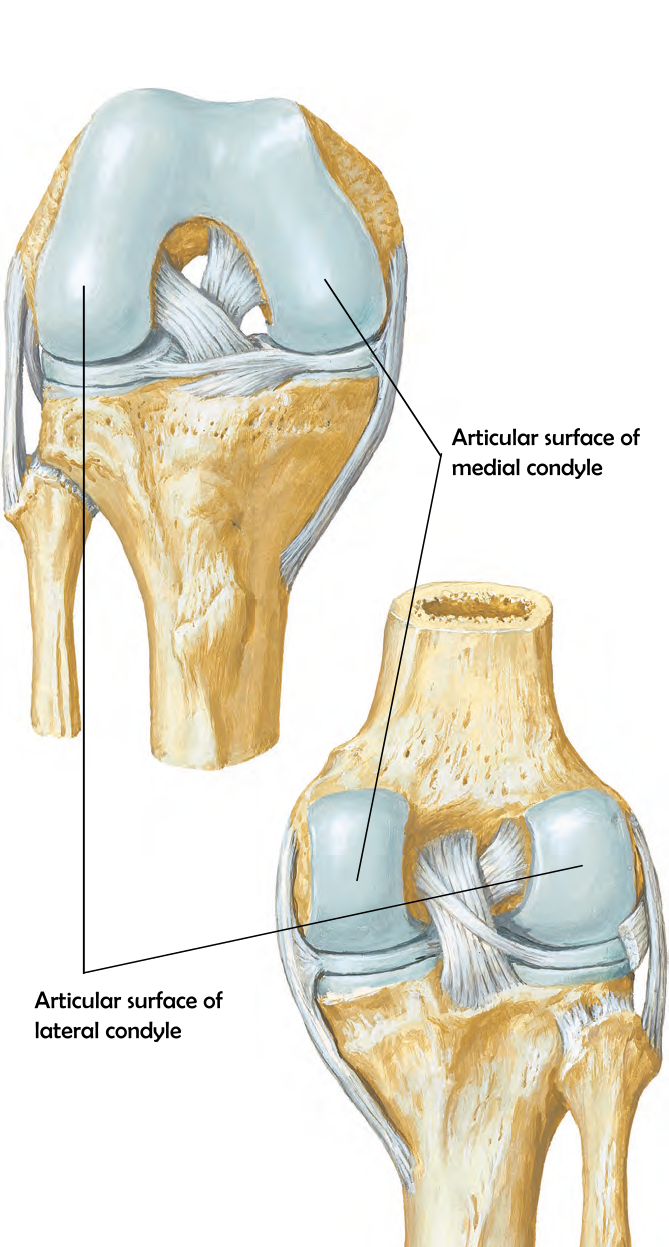
\includegraphics[scale=0.3]{right_knee_labeled}
	\caption{Anterior (top, showing the knee in flexion) and posterior (bottom, showing the knee in extension) views of the right knee, with labeled articular surfaces of the medial and lateral condyles. [Edited] \parencite[p.519]{netter_519_2023}}
	\label{fig:rightkneeplate519}
\end{figure}

\begin{figure} [H]
	\centering
	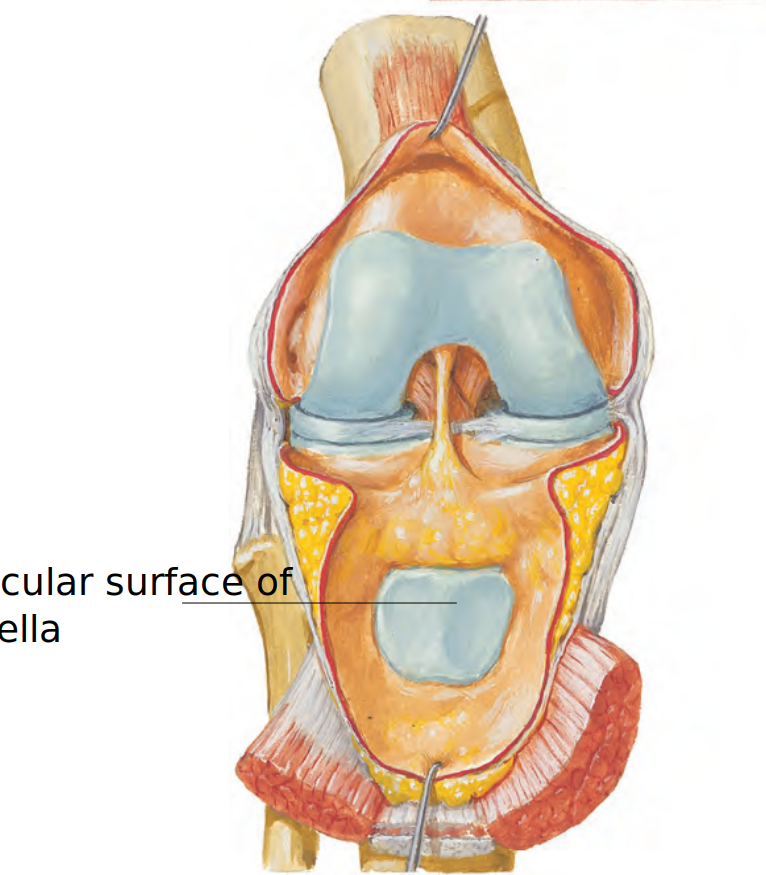
\includegraphics[scale=0.3]{patellar_surface}
	\caption{Right knee joint opened, with the knee in a slightly flexed position, exposing the articular surface of the patella.[Edited] \parencite[p.517]{netter_519_2023}}
	\label{fig:patellarsurface}
\end{figure}

This design allows the knee to manage a wide array of movements and bear significant loads. Figure \ref{fig:sixdegrees} illustrates the knee's capacity for multidimensional movement, highlighting the joint's sophisticated structural design that enables this versatility. However, this inherent design also renders the knee vulnerable to a range of forces, including compressive forces acting on bone and cartilage, tensile stresses in periarticular ligaments, and substantial muscular forces required to maintain balance during weight-bearing activities. \parencite{standring_grays_2021} For instance, during symmetrical stance on both feet, each knee supports approximately 43 \% of the body's weight, necessitating precise muscular coordination to maintain equilibrium \parencite{maquet2012biomechanics}.

\begin{figure}[H]
	\centering
	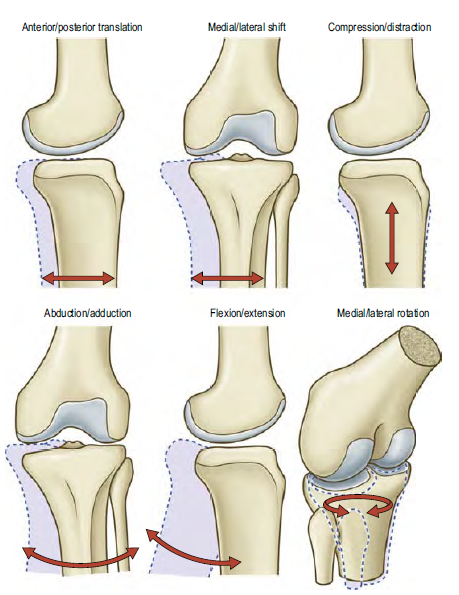
\includegraphics[width=0.7\linewidth]{six_degrees}
	\caption{The knee joint motion in three dimensions, described using six degrees of freedom: anterior/posterior translation, medial/lateral shift, compression/distraction, abduction/adduction, flexion/extension, and medial/lateral rotation. The arrows indicate the direction of each movement. \parencite[p.~1412]{standring_grays_2021}.}
	\label{fig:sixdegrees}
\end{figure}

Such mechanical forces, influenced by activities and body mass index (BMI), are significant causes of OA and represent one of the most modifiable risk factors \parencite{heidari_knee_2011}. Both static and dynamic forces play critical roles in the pathophysiology of OA. Static forces, such as those experienced while standing, contribute significantly to mechanical stress on the knee joint, exacerbating the risk of OA \parencite{egloff_biomechanics_2012}. Additionally, abnormal joint loading during movement is a key mechanical driver of osteochondral changes that contribute to the initiation and progression of knee OA \parencite{coburn_immediate_2023}.


The relationship between biomechanical stresses and knee health highlights the need for diagnostic tools that fulfill two key criteria: they must capture the knee's dynamic behavior during motion and assess the joint under varying loads. Dynamic MRI is emerging as a notable imaging modality that meets these criteria \parencite{conconi_-vivo_2023}. 


\subsection{Dynamic MRI}
In a broad sense, dynamic MRI is an umbrella term encompassing various MRI techniques designed to capture and visualize physiological processes and motion over time. The dynamic aspect of MRI is crucial for studying systems or structures involving inherent motion, such as blood flow, tissue perfusion, or cardiac activity. For the purposes of this project, the focus of "dynamic MRI" narrows down to capturing the bulk movement of the knee joint undergoing active flexion extension cycles inside the scanner. Compared to traditional static MRI scans, which are highly susceptible to motion artifacts compared to other imaging modalities \parencite{zaitsev_motion_2015}, dynamic MRI techniques not only accommodates motion, but can even leverage it to offer comprehensive insights into the functional and biomechanical properties of the concerned structures.  Among these techniques, CINE imaging, particularly renowned in cardiac MRI, is considered the gold standard for evaluating cardiac function \parencite{menchon-lara_reconstruction_2019}. Its high regard in cardiac MRI demonstrates the method's precision and adaptability—traits that are leveraged in knee imaging.

\subsubsection{CINE imaging}

The word CINE, derived from 'cinematography,' refers to creating a movie-like sequence of images. In the context of dynamic knee MRI, this technique can be used to reconstruct a "movie" of a single flexion/extension cycle. This visualization is achieved by aggregating multiple partial datasets acquired over various cycles. The knee's movement cycle is segmented into distinct stages, each corresponding to a specific angle of flexion or extension. For each stage, k-space — the Fourier transform space from which MR images are reconstructed — is incrementally sampled. This data is gathered across multiple repetitions of the movement cycle, ensuring comprehensive coverage of k-space and thus, high-resolution imaging of each movement phase.This technique works robustly only if the movement cycles of the knee during imaging are sufficiently similar to each other \parencite{curtis_primer_2022}. Achieving this consistency in dynamic MRI of the knee, which naturally involves significant movement variations, requires precise synchronization of the imaging process with the knee's motion cycle. 

\subsubsection{Gating} 

This synchronization, known as gating, aligns image acquisition with specific, repeatable points in the knee's movement cycle. By synchronizing image acquisition with specific phases of the knee's movement cycle, gating allows for accurate reconstruction of the dynamic motions of the knee, enabling precise biomechanical analyses. There are two main types of gating: retrospective and prospective. In prospective gating, image acquisition is triggered at specific points in the motion cycle in real-time. For this project, retrospecting gating is used, where the data is acquired continuously throughout the motion cycle \parencite{edelman_clinical_1996} and then reordered post-acquisition into a coherent sequence that captures the knee at different positions along the motion cycle. This necessitates external information that captures the precise moment and position of the knee throughout its range of movement beyond just the raw data acquired during the MRI scan. A MR-safe knee loading device is employed to address this, which comes with an optical sensor attachment that provides this vital information that includes the exact timing and degree of knee flexion and extension \parencite{brisson_novel_2022}. 

\subsubsection{Knee loading device }

The MR-compatible knee loading device employed in this study is illustrated in Figure \ref{fig:kneedevice}. This device allowed for a range of motion of approximately 25 to 45 degrees (subject-dependent), enabling subjects to perform knee flexion and extension cycles under both loaded and unloaded conditions. For loading, the device is equipped with compartments for weight plates and sandbags, providing a physiological load of 10 to 12 kilograms. These weights are positioned at the end of the device near the subject's lower limb. As the subject extends the leg, they must overcome not only the natural inertia of their body weight but also the additional external load imposed by these weights. Similarly, as the subject flexes the leg from the extended position, they have to lower the leg in a controlled manner which also requires effort. 

Central to this device's functionality is an optical fiber position sensor (MR338-Y10C10, Micronor, 155 Camarillo, CA, USA), which precisely  measures the ab­solute angle from 0{\degree}\,to 360\degree \, with a resolution of 0.025\degree \parencite{rickenbach_optical_2013}. This measurement capability is critical for synchronizing the knee's movement with MRI data reconstruction. 
\begin{figure} [H]
	\centering
	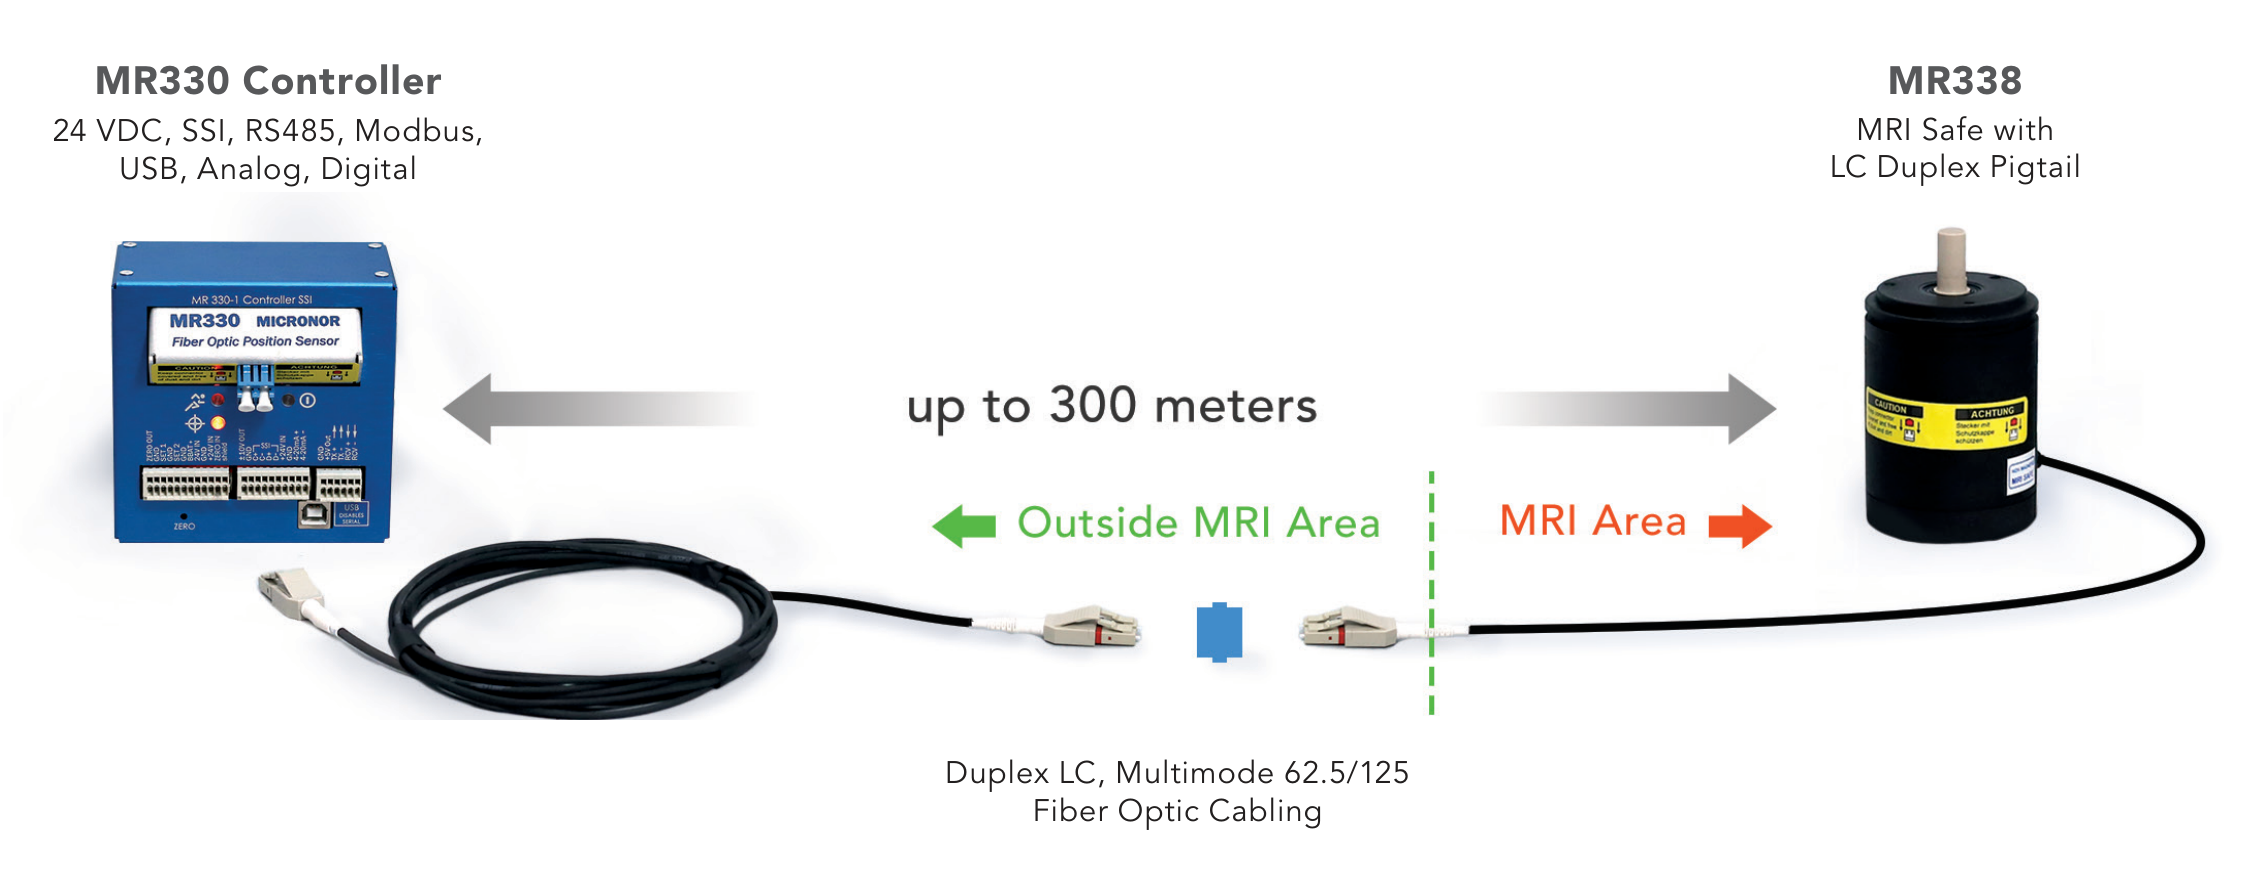
\includegraphics[width=0.7\linewidth]{sensor_img}
	\caption{The MR330 controller (left) and MR338 optical fiber position sensor system (right), connected via duplex LC multimode fiber optic cabling, with a maximum distance of up to 300 meters. The setup illustrates the separation between the outside MRI area and the MRI-safe area.}
	\label{fig:sensorimg}
\end{figure}


As shown in Figure \ref{fig:sensorimg} , the MR330 controller interfaces with the MRI-safe MR338 position sensor to facilitate precise measurement within the MRI environment, accommodating up to 300 meters of fiber optic cabling. The controller is connected to a acquisition computer placed outside the scanner while the sensor is attached to the device within. The MR338 rotary encoder continuously monitors the knee's rotation angle using optical signals, which are converted into electrical signals by the MR330 controller. These electrical signals are then sent to the RedLab 1208LS (Meihaus Electronic GmbH), a USB-based data acquisition module designed for measuring analog and digital signals (refer to Figure \ref{fig:redlab}). The MRI scanner outputs trigger signals for each sequence repetition as a voltage signal, which are also captured by the RedLab 1208FS-Plus. Both the knee rotation signals and the trigger signals are simultaneously sampled by the RedLab 1208FS-Plus and then transmitted to the acquisition computer via USB. The acquisition computer converts these signals into binary data, which is later used for reconstructing the synchronized knee motion and MRI imaging data.  
\begin{figure}[H]
	\centering
	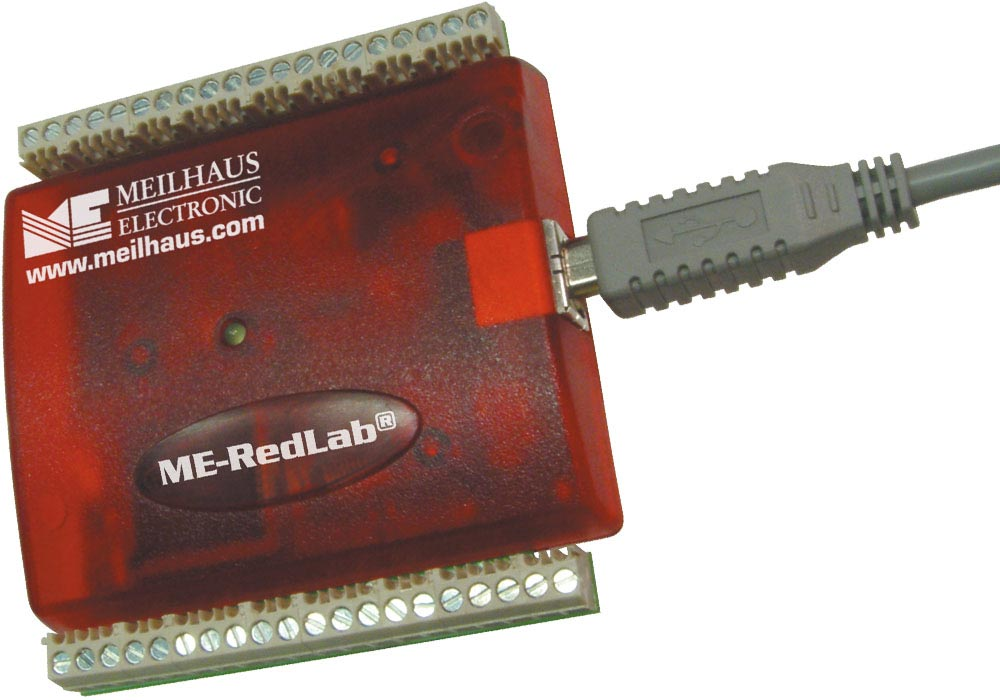
\includegraphics[scale=0.1]{redlab}
	\caption{The RedLab 1208LS module, a USB data acquisition device by Meihaus Electronic GmbH. This unit, shown with attached USB cable, converts optical to electrical signals for MRI applications}
	\label{fig:redlab}
\end{figure}




To enhance signal acquisition and the clarity of imaging, two flexible coils (Noras, Variety) as shown in Figure \ref{fig:coils} were positioned at key anatomical locations: one at the distal femur and another at the proximal tibia, as specified in the MRI protocol. 

\begin{figure}[H]
	\centering
	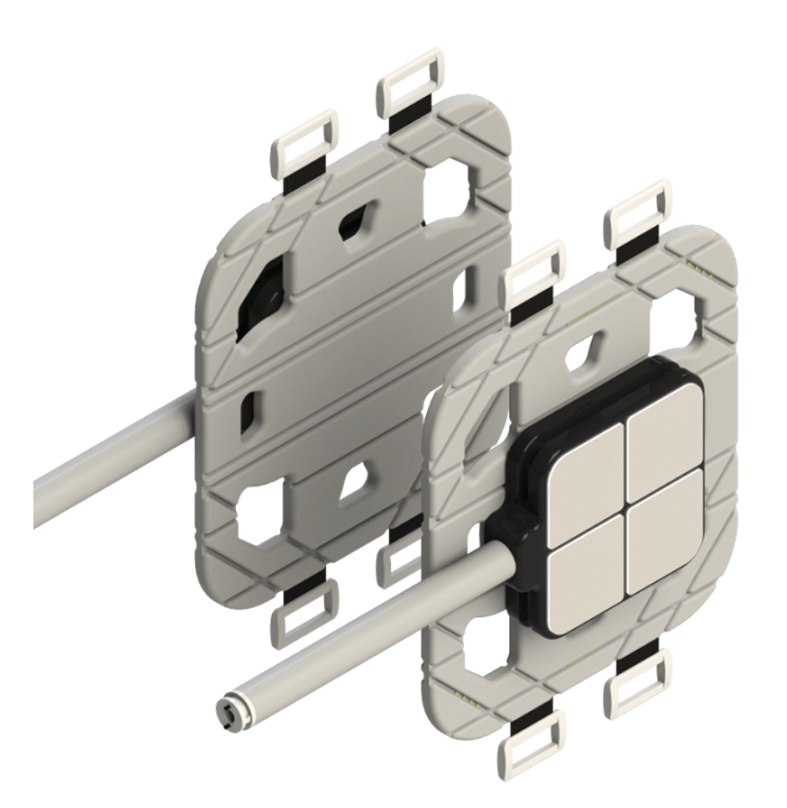
\includegraphics[scale=0.2]{coils}
	\caption{Noras Variety 16 channel flex coils, designed for MRI applications. The image shows the flex coil with a central square exterior featuring Velcro for secure strapping, highlighting its flexible design}
	\label{fig:coils}
\end{figure}


\begin{figure}[H]
	\centering
	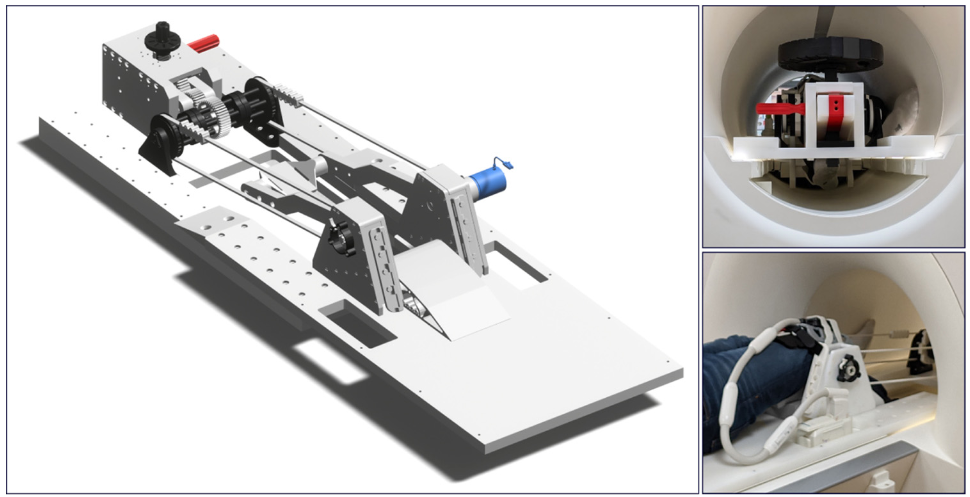
\includegraphics[width=0.9\linewidth]{knee_device}
	\caption{"A 3D rendering of the knee motion/loading device (left) and two photographs of the device in a Siemens Magnetom Prisma Fit MRI scanner (right). The top right image (rear view) demonstrates how the distal part of the device sits atop the rails within the scanner bore, which are normally used to guide and support the patient table. The bottom right image (front, oblique view) demonstrates an individual positioned in the device with a flexible coil around the index knee, the thigh secured between the proximal pillow blocks and the ankle fastened to the leg support, as well as the coil plug setup" \parencite{brisson_novel_2022}. }
	\label{fig:kneedevice}
\end{figure}
 


  
To further enhance the quality and precision of the imaging, and to maximize the potential for precise image reconstruction, a previously reported radial golden-angle gradient-echo Fast Low-Angle Shot (FLASH) sequence was used, which is more robust against motion artifacts than Cartesian sequences \parencite{aleksiev_high-resolution_2022}. The following sections will detail the key components of this technique — radial golden-angle acquisition and the gradient-echo FLASH sequence.

\subsubsection{Gradient Echo FLASH sequence}

\textbf{Basics}

At its core, MRI is an imaging technique based on the interaction of nuclear spins with an external magnetic field \textbf{($B_0$)}. The primary nucleus used in MRI is the proton in hydrogen, which precesses around the direction of this external field.  When placed in the magnetic field, these protons align with or against the direction of \textbf{$B_0$}, creating a net magnetization vector \textbf{$M_z$} along the field direction. Imaging the human body relies on manipulating and detecting the bulk precession of these hydrogen spins in water, fat, and other organic molecules \parencite{brown_magnetic_2014}. This manipulation is achieved through various sequences of magnetic field gradients, radiofrequency pulses, and timing sequences. 


One such commonly used sequence is the gradient echo (GRE) sequence. Like any other sequence, the process begins with the application of a radiofrequency (RF) pulse. This RF pulse is an oscillating magnetic field applied at the Larmor frequency, which is the natural precession frequency of the hydrogen protons in the magnetic field. This frequency $\omega_0$ is given by the Larmor equation:
\begin{equation}
	\omega_0 = \gamma B_0
	\label{eq:larmor}
\end{equation}
where $\gamma$ is the gyromagnetic ratio and $B_0$ is the external magnetic field.
When the frequency of the RF pulse matches the Larmor frequency, it resonates with the protons, causing the net magnetization vector \textbf{$M_z$} to tip from the longitudinal axis into the transverse plane, creating a transverse magnetization \textbf{$M_{xy}$}. This is where the term "resonance" in Magnetic Resonance Imaging originates. 

\textbf{$M_{xy}$} generates the detectable MRI signal by inducing an oscillating voltage in the receiver coils, which is known as free induction decay (FID). However, to form a meaningful image, it is essential to encode spatial information within this signal. This spatial encoding is achieved through the use of gradient magnetic fields applied in various directions. These gradients alter the precession frequencies of the protons based on their spatial positions, allowing the mapping of the location of the signals within the body.  

\textbf{The three gradient fields}

The first gradient field applied is the slice-selecting gradient ($G_{SS}$). It is applied in the direction of \textbf{$B_0$}, simultaneously with the application of the RF pulse. 
This gradient varies the magnetic field strength along the z-axis, causing the protons to precess at different frequencies according to equation \ref{eq:larmor}. As a result, only the protons at a specific location along the z-axis, where their Larmor frequency matches the RF pulse frequency, will resonate and be tipped into the transverse plane, thereby selecting a specific slice for imaging. Immediately after the RF pulse and $G_{SS}$, a rephasing gradient with opposite polarity in the slice-selecting direction is applied. The purpose of this rephasing lobe is to correct for any dephasing caused by the initial  $G_{SS}$. When the initial gradient is applied, protons within the selected slice experience slightly different magnetic field strengths, causing them to dephase. The rephasing gradient lobe reverses this effect by applying a gradient of the same magnitude but opposite polarity, bringing the spins back into phase within the selected slice. This ensures that \textbf{$M_{xy}$} is coherent, maximizing the strength of the detectable signal.

Once the slice is selected, signal localization along the remaining two perpendicular directions in the transverse plane must be performed. The process begins with frequency encoding. Another gradient field, lets say in the x-direction, called the frequency encoding gradient (\textbf{$G_{FE}$}), is applied simultaneously during signal acquisition. When this gradient is applied, protons experience different precession frequencies based on their spatial location along the x-axis. The sampled signal will be a superposition of these frequencies, which can be resolved by performing an inverse Fast Fourier Transform (FFT) to reconstruct the spatial information along the x-direction. Before the main \textbf{$G_{FE}$} is applied during acquisition, a gradient of opposite polarity, known as the prephasing gradient, is briefly applied. This prephasing gradient slightly dephases the spins, establishing a known initial phase relationship. When the main frequency encoding gradient is subsequently applied, it causes the spins to rephase, forming an echo signal at a specific time. This rephasing process generates the "gradient echo," which is the reason for naming this sequence as it is. The prephasing gradient is typically shorter and is followed by the longer main frequency encoding gradient, ensuring that the spins are coherently rephased at the start of signal acquisition, maximizing the strength of the detected signal.

Next, phase encoding is performed to spatially encode information along the second perpendicular (y) direction. The phase encoding gradient \textbf{($G_{PE}$)} is briefly turned on and then off before $G_{FE}$ is applied. During the time $G_{PE}$ is on, the spins start precessing at different frequencies based on their spatial location along the y-axis, causing them to dephase. When $G_{PE}$ is turned off, the spins return to precessing at the Larmor frequency, but the phase differences induced by the gradient remain. 

After this initial encoding, the same sequence is repeated multiple times. Each repetition is identical except for the magnitude of the phase encoding gradient $G_{PE}$, which is varied systematically. By altering the strength of $G_{PE}$ in each repetition, different phase shifts are induced, corresponding to different spatial locations along the y-axis. This process effectively samples the spatial information across the entire y-direction. The collected data from these repetitions fill what is known as k-space, a matrix that represents the spatial frequency domain of the image. Each line in k-space corresponds to a different phase encoding step. Once k-space is fully sampled, an inverse FFT is performed to convert the frequency-domain data into a spatial-domain image. This combination of frequency encoding and phase encoding allows for the reconstruction of a two-dimensional image of the selected slice.

\textbf{FLASH}

The refocusing gradient used in gradient-echo pulse sequences allows for significantly shorter echo times (TE), facilitating faster imaging \parencite[p.94]{westbrook_mri_2019}. However, certain applications, such as dynamic MRI of moving body parts like the leg, demand even quicker acquisition times. To meet these demands, the Fast Low Angle Shot (FLASH) GRE sequence was developed \parencite{haase_flash_1986}. FLASH employs low flip angle RF pulses, which reduce the time needed for the longitudinal magnetization to recover, thereby shortening the repetition time (TR). 

Another important aspect of FLASH sequences is the management of residual transverse magnetization. In gradient echo sequences, after a series of RF pulses, the system reaches a condition known as the steady state. In this state, the magnitude of $M_z$ remains consistent at the end of each TR. However, there can also be residual $M_{xy}$ at the start of each repetition cycle. If this residual transverse magnetization is not managed, it can interfere with the signal and degrade image quality. To address this, FLASH sequences incorporate a strong spoiler gradient in the slice-selecting direction. This gradient deliberately dephases the residual transverse magnetization, ensuring that it does not contribute to the signal in subsequent cycles. By effectively "spoiling" the transverse magnetization, the sequence starts fresh with each repetition, reducing artifacts and enhancing image clarity.

A typical FLASH sequence diagram is shown in Figure \ref{fig:gresimplified}, illustrating the application of low flip angle RF pulses, frequency encoding gradients, and the spoiler gradient.

\begin{figure}[H]
	\centering
	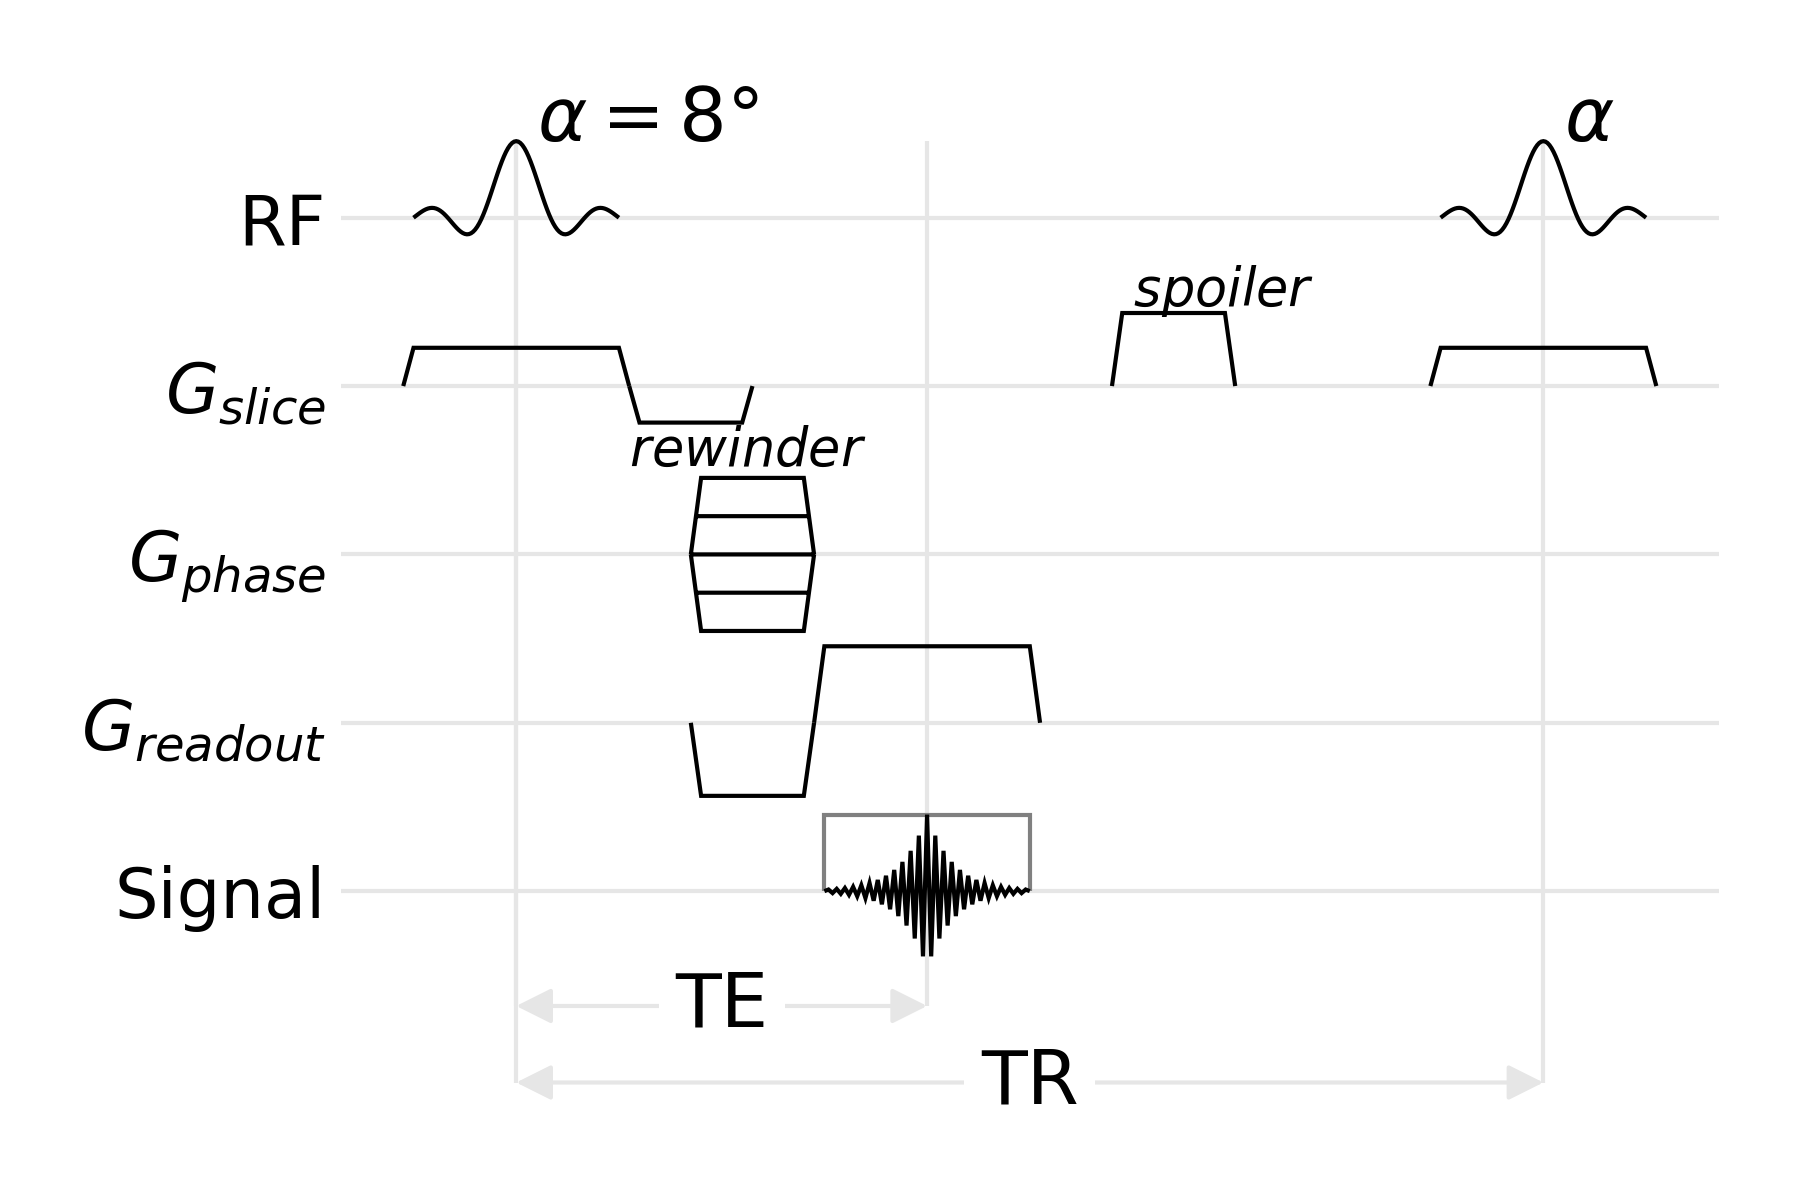
\includegraphics[width=0.7\linewidth]{flash_seq}
	\caption{FLASH sequence diagram. The diagram illustrates the key components of the FLASH sequence: RF Pulse with flip angle $\alpha^\circ$, Slice-Selecting Gradient ($G_{SS}$), Phase Encoding Gradient ($G_{PE}$), Frequency Encoding Gradient ($G_{FE}$), Signal, and Spoiler Gradient, echo time (TE) and repetition time (TR)}
	\label{fig:gresimplified}
\end{figure}

\subsubsection{Radial golden-angle acquisition}


Radial golden-angle acquisition refers to the modification in how k-space is sampled. Unlike traditional static MRI, which typically employs Cartesian line by line sampling, this method utilizes radial sampling. Here, the data points are collected along radial lines spreading out from the center of k-space, resembling spokes on a wheel. Figure \ref{fig:radial} depicts a generic radial sampling scheme. The separation between any two adjacent circles defines the separation $\Delta k_r$ in the radial sampling direction, whereas, the angular separation between any two successive angular lines in k-space (such as between the two example lines shown in the figure) defines $\Delta \theta$. The two quantities $\Delta k_r$ and $\Delta \theta$ are constrained by the Nyquist sampling criterion. \parencite{brown_magnetic_2014} 
  
 \begin{figure}[H]
 	\centering
 	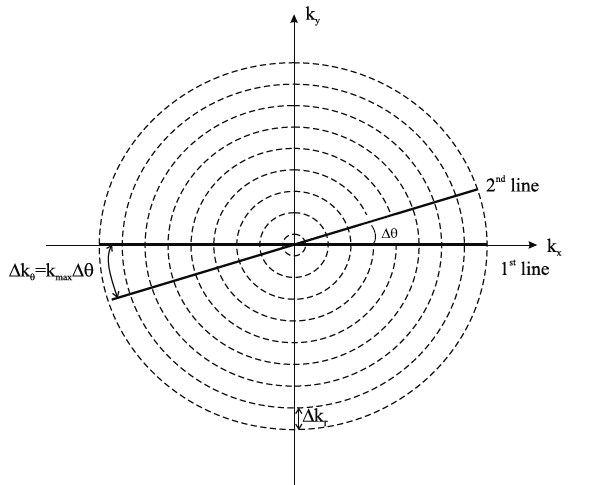
\includegraphics[width=0.7\linewidth]{radial}
 	\caption{Generic radial k-space sampling diagram. The image shows concentric circles representing constant k-space radii, with $k_x$ and $k_y$ axes indicating spatial frequencies. The lines labeled '1st line' and '2nd line' demonstrate different radial sampling lines, each separated by an angle $\Delta \theta$. The equation $\Delta k_{\theta} = k_{\text{max}} \Delta \theta$ illustrates that the change in the k-space coordinates along a specific angular direction ($\Delta k_{\theta}$) is proportional to the maximum k-space radius ($k_{\text{max}}$), which determines the highest spatial frequency sampled, and the angular step size ($\Delta \theta$).
 		 \parencite[p.306]{brown_magnetic_2014}}
 	\label{fig:radial}
 \end{figure}
 
 The 'golden-angle' strategy, which was used in this work, optimizes this approach by spacing the radial lines at an angle of approximately 111.25 degrees. This specific angle helps in continuously covering the k-space without overlapping lines, ensuring that each new image frame provides unique information, thus enhancing image quality and temporal resolution. 
 
\begin{figure}[H]
	\centering
	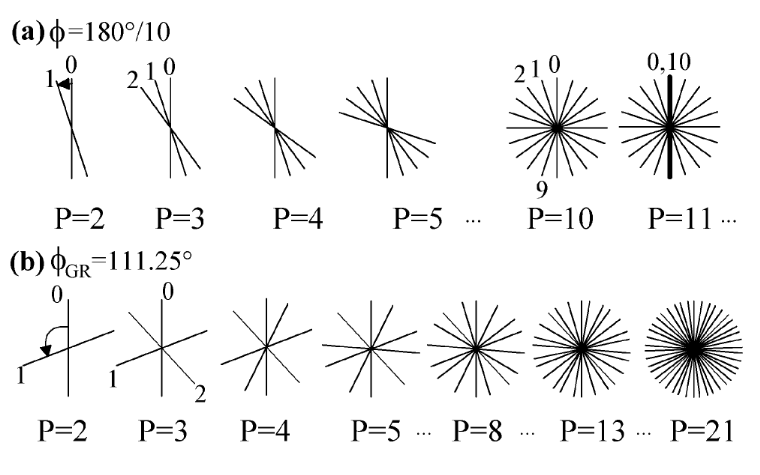
\includegraphics[width=0.7\linewidth]{golden_angle_figure}
	\caption{Radial k-space sampling strategies. (a) Fixed angular increment ($\phi = 180^\circ / 10$), showing potential for uneven k-space coverage. (b) Golden-angle sampling ($\phi_{GR} = 111.25^\circ$), ensuring uniform distribution across k-space as the number of projections ($P$) increases \parencite{winkelmann_optimal_2007}.}
	\label{fig:goldenanglefigure}
\end{figure}

 
Figure \ref{fig:goldenanglefigure} provides a visual comparison between traditional fixed increment and the golden-angle methods in k-space sampling. It highlights how each approach affects the distribution of sampling lines across k-space. In the figure, part (a) shows radial sampling using a fixed angular increment. This traditional method can lead to gaps or overlaps in data collection, depending on the number of radial profiles used. Part (b) demonstrates the golden-angle method, where each new radial line is placed at an increment of approximately 111.25 degrees. This approach allows for a more uniform distribution of sampling lines across k-space, enhancing image quality by preventing gaps and reducing redundancy in data collection. Figure \ref{fig:kspacearrow} is an example of the k-space data acquired during a specific frame of the knee flexion cycle along with  the reconstructed MRI image in real space obtained by applying an inverse 2D Fast Fourier Transform (2D IFFT) to the k-space data.
\begin{figure}[H]
	\centering
	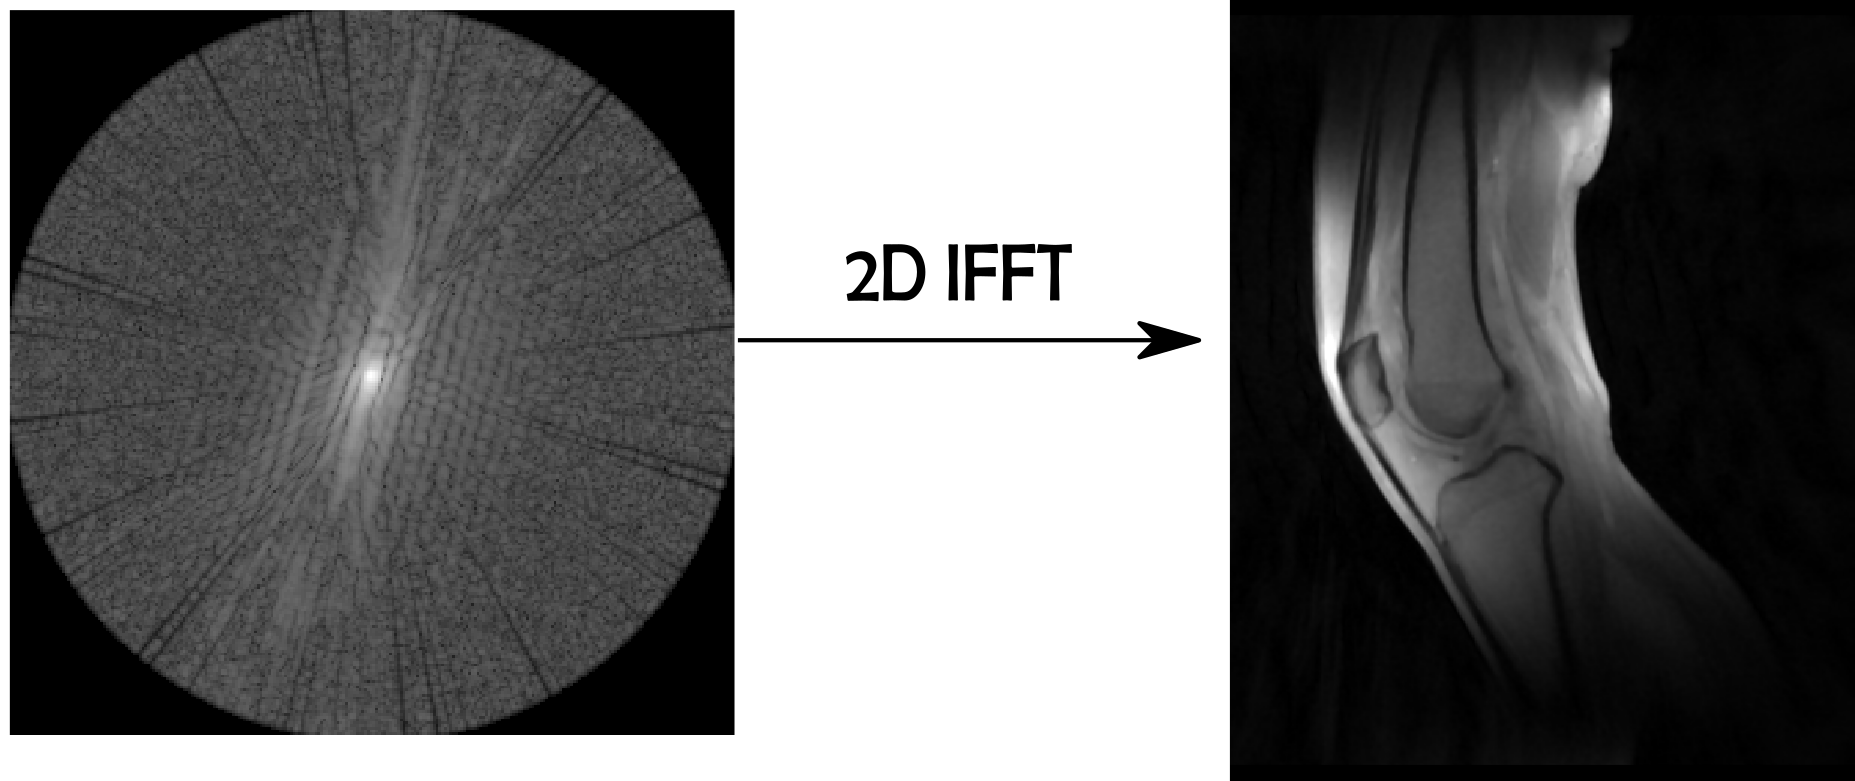
\includegraphics[scale=0.3]{kspace_arrow_2}
	\caption{Left: Exemplary magnitude of k-space data acquired during a specific frame of the knee flexion cycle. Right: Reconstructed MRI image in real space obtained by applying an inverse 2D Fast Fourier Transform (2D IFFT) to the k-space data}
	\label{fig:kspacearrow}
\end{figure}
  


\section{Methodology}
\label{sec:second}

\subsection{Data Collection Methods}

\subsubsection{Procedure Details}
Dynamic MRI scans were conducted on five healthy individuals, two females and three males, ranging in age from 28 to 39 years and weighing between 55 to 90 kilograms, utilizing a 3 T Siemens Prisma scanner. These volunteers were free from any known musculoskeletal disorders and provided their written consent, adhering to the ethical standards approved by the institutional review board. For all of these subjects, the left leg was scanned. 


Once the subject was positioned supine in the scanner, the thigh was secured on a wedge positioner with a strap, and the lower leg was attached to an ankle rest, just above the malleoli, using Velcro straps to minimize lateral movement. The knee to be examined is aligned with the device’s axis of rotation, while the other leg rests alongside the MRI scanner's bore.  Knee motion is guided by a belt and sprocket assembly running alongside the lower leg, connected to a gearbox activated by the leg support as the participant flexes and extends the knee. Once the subject was positioned at the scanner's isocenter, their leg naturally assumed a flexed posture due to the design of the device. In this configuration, the leg is cradled by the device arm which is positioned below the level of the knee, ensuring that the leg remains flexed without the volunteer exerting any force.


The volunteer engaged in a controlled exercise, following a metronome set at 60 beats per minute. This pace dictated a four-beat flexion to extension cycle, with the leg being flexed at the first beat and fully extended by the fourth. This equals to 8 beats per cycle, or 7.5 cycles every minute. Initially conducted under a loaded condition, the process was repeated without the added resistance to compare both states. The scan duration was 160 seconds, amounting to 20 full flexion-extension-flexion cycles. The range of motion for each dataset is noted in table \ref{tab:range_of_motion}. 

\begin{table}[H]
	\centering
	
	\caption{Range of Motion for Different Datasets}
	\label{tab:range_of_motion}
	\begin{tabular}{cc}
		\toprule
		Dataset & Range of Motion (°) \\
		\midrule
		1 & 38 \\
		2 & 30 \\
		3 & 36 \\
		4 & 36 \\
		5 & 46 \\
		\bottomrule
	\end{tabular}
	
	
\end{table}

\subsubsection{Sequence Parameters and Reconstruction}
Table \ref{tab:mri_seq_params} lists the MRI sequence parameters:

\begin{table}[H]
	\centering
	
	\caption{MRI Sequence Parameters}
	\label{tab:mri_seq_params}
	\begin{tabular}{@{}ll@{}}
		\toprule
		Sequence Parameters & Values \\ \midrule
		Acquisition Duration & 160 [s] \\
		Dwell Time & 0.0024 [ms] \\
		Echo Time & 2.51 [ms] \\
		Field Strength & 2.89362 [T] \\
		Flip Angle & 8.0 [deg] \\
		Field of View (FOV) & 192.0 x 192.0 x 3.0 [mm] \\
		Frequency & 123.25 [MHz] \\
		Inversion Time & 150000 [ms] \\
		Matrix Size & 176 x 176 x 1 \\
		Repetition Time & 5.8 [ms] \\
		\bottomrule
	\end{tabular}
\end{table}

In this study, the k-space data was acquired using 16 receive channels, each recording data simultaneously but with a unique spatial sensitivity profile. 276 spokes used to sample one full k-space. With a TR of 5.8 milliseconds per spoke, it took approximately 1.6 seconds to acquire one k-space. Over the course of the experiment, 100 such k-space repetitions are acquired, equaling 100 repetitions as noted. The total scan duration either under loaded or unloaded condition was 160 seconds. Based on participant feedback, this duration was reported as being manageable to perform the exercise. 

Each acquired k-space repetition contained data across a range of knee flexion angles because of the continuous leg movement set to the metronome beat. Assuming subjects perform perfectly in time at 60 beats per minute, it takes 4 seconds to move the leg from maximum flexion to full extension. Since one k-space acquisition took 1.6 seconds, this duration is not enough to capture sufficient data to fully reconstruct frames at any specific flexion angle. Therefore, to reconstruct the full range of knee angles accurately,  100 k-space repetitions were acquired. 
    
\textbf{Reconstruction}

The MRI raw data, with dimensions of (352, 276, 16, 100), was processed using a reconstruction pipeline to generate the final image dataset. These dimensions correspond to: 
\begin{itemize}
	\item 352: The number of data points per spoke.
	\item 276: The number of spokes used to sample a k-space dataset.
	\item 16: The number of receive channels
	\item 100: The number of k-space repetitions acquired over the course of the experiment.
\end{itemize}

In addition to the raw MRI data, the binary data from the acquisition computer, which includes both the optical sensor readings and MRI scanner trigger signals, was loaded. This binary data was read and parsed to extract the knee rotation angles (in degrees) and the MRI trigger signals in a usable format. By detecting significant changes in the trigger signals, the start of new k-space repetitions were identified. The knee rotation angles were then grouped according to each k-space repetition based on these trigger signals. This resulted in 100 groups, each containing a range of knee rotation angle information for a specific k-space repetition. 

For each k-space repetition, the spokes were categorized based on the knee rotation angles, divided into 2-degree intervals. This means each reconstructed frame covered a 2-degree segment of knee motion. This process was repeated for the entire range of motion, ensuring a comprehensive coverage.  

Image reconstruction was then performed on each newly formed k-space dataset. The number of spokes within each 2-degree angle range varied between 300 and 1000. The direction of leg movement—either flexion, where the leg moves downward, or extension, where the leg moves upward—was determined by calculating the slope of the angle data. Images were reconstructed separately for each direction, as the biomechanics of moving downward (flexion) versus upward (extension) differ significantly.  

\textbf{Non cartesian image reconstruction (RIESLING)}

Iterative image reconstruction is a computational method used in various imaging modalities, including MRI, to enhance image quality. Unlike direct reconstruction techniques, iterative methods repeatedly refine the image by comparing the acquired data with an estimated version of the image, making adjustments to minimize the difference between the two. This process allows for better handling of incomplete or noisy data, improving the accuracy and resolution of the final image. Iterative reconstruction is particularly advantageous in non-Cartesian MRI because it can effectively manage the complex data geometry, leading to more precise and detailed images \parencite{block_undersampled_2007}.

To implement these iterative reconstruction methods, the actual image reconstruction was done by using the RIESLING (Radial Interstices Enable Speedy Low-Volume imagING)   reconstruction toolbox \parencite{wood2020riesling}. This toolbox offers a range of advanced algorithms tailored for non-Cartesian MRI reconstruction. In this study, an Alternating Direction Method of Multipliers (ADMM) approach was employed \parencite{MAL-016}, incorporating Total Generalized Variation (TGV) regularization \parencite{tgv}. 

ADMM is an iterative optimization algorithm that breaks down complex problems into smaller subproblems to solve them efficiently. It ensures accurate reconstruction by maintaining a balance between the primal (actual solution) and dual (approximate solution) residuals. This balance is particularly important for non-Cartesian MRI reconstruction, given the unique geometry of the data. ADMM allows different regularization techniques, like TGV, to be applied simultaneously during reconstruction . 

TGV is an advanced regularization method that reduces noise while promoting smoothness in the reconstructed images. Unlike basic Total Variation (TV) regularization, TGV allows for piecewise smooth transitions between different regions, making it better suited for images with varied structures. In this study, a regularization strength of 0.05 was chosen empirically, striking a balance between noise suppression and edge sharpness.

Each image frame was reconstructed with dimensions of (528, 528) and the number of frames were subject dependent directly influenced by their range of motion achieved within the scanner bore.


\subsection{Data Analysis}
All analyses and data visualization were done using the python programming language (v3.11.5). Several distinct steps were performed to semi-automate the segmentation of tibia and femur. This involves first finding one boundary edge each for the bones, and then tracking them across the full flexion-extension cycle by computing their respective transformation matrices. 
 
\subsubsection{Segmentation}
The semi-auto segmentation process is achieved in five distinct steps as described below: 

\textbf{Step 1: Edge Detection}

The Canny filter \parencite{canny_computational_1986}, as implemented in the scikit-image's feature library (v0.21.0), was employed to apply an edge filter to the images. The Canny edge detection algorithm operates in several key steps to identify edges with high accuracy in images. Initially, the image is smoothed using a Gaussian filter to reduce noise and potential false edge detections. Following this, the algorithm calculates the gradient intensity and direction of the image brightness at each pixel, which helps in identifying the edges' boundaries. This is done by differentiating the image in two orthogonal directions and computing the gradient magnitude as the root sum of
squares of the derivatives. The gradient direction is computed using the arctangent of the ratio of the derivatives.

Subsequently, the algorithm applies double thresholding, which involves two thresholds: a low and a high. This creates three categories of pixels: strong, weak, and non-edges. Pixels with intensities above the high threshold are marked as strong edge pixels, while those below the low threshold are considered to be non-edges. Pixels between these two thresholds are marked as weak edge pixels. Weak edge pixels are potentially converted into strong edges through a process known as hysteresis, where only those weak edges that are connected to strong edges are confirmed as true edges. In this context, hysteresis refers to the algorithm's reliance on the connectivity history of pixels to decide their edge status, ensuring that only meaningful, connected edges are preserved \parencite{heath_robust_1997}.  

To optimize the edge detection specifically to capture the desired edges of the tibia and femur, different parameters like the standard deviation of gaussian blur ($\sigma$) and the upper and lower thresholds were tested in different combinations. The optimal results were achieved with a low threshold between 0 to 5 and a high threshold between 6 to 10. and a value of 2 was used for $\sigma$. Figure \ref{fig:edgemitimg} displays the output of the edge detection with these parameters.  
\begin{figure}[H]
	\centering
	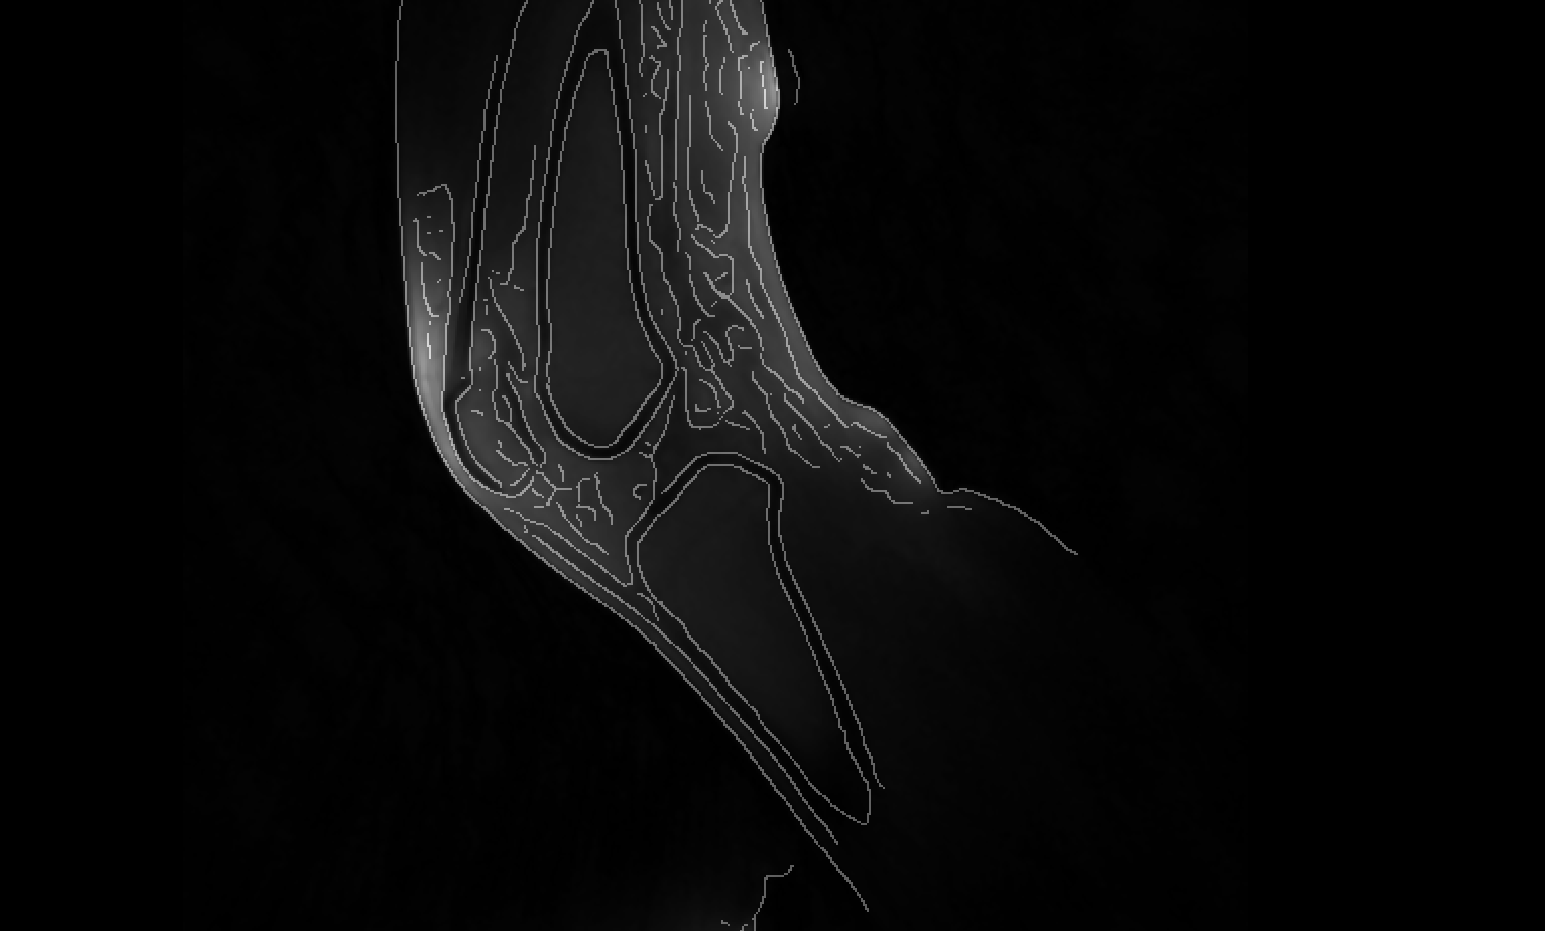
\includegraphics[width=0.7\linewidth]{edge_new}
	\caption{Output of the Canny edge detection algorithm applied to one of the frames, showing the detected edges (white) overlayed on top of the original image for visual comparison.}
	\label{fig:edgemitimg}
\end{figure}


Subsequently, the scikit-image's morphology library was utilized to remove small elements from the binary image. The image was then skeletonized to a one-pixel width, retaining only long and consistent edges. It should be pointed out that the final edge does not necessarily need to span the full boundary of the interior edge of the cortical bone; even partial edges were successfully used for this purpose.  

\textbf{Step 2: Labelling}

For the final selection of the desired edges, a labeling algorithm (`ndimage.label`) from SciPy, an open-source Python library designed for scientific computing (version 1.11.3), was utilized. The purpose of employing this labeling algorithm is to effectively isolate specific structural features, such as distinguishing the interior cortical bone from the exterior, by assigning unique labels to separate closely situated edges detected in the image. This algorithm applies the principle of connected-component labeling, a method used in computer vision to detect connected regions in binary digital images \parencite{dillencourt_general_1992}. Connected-component labeling algorithm scans an image and groups its pixels into components based on pixel connectivity, meaning that all pixels in a connected component share similar pixel values and are adjacent to each other.

The labeling process treats any non-zero values in the input array as part of potential edges and zero values as background. The connectivity of these components is determined by a structuring element, which in this case was a fully connected $3\times3\times3$ matrix. This structuring element ensures that each voxel (3D pixel) is connected to its 26 immediate neighbors (including those connected by faces, edges, and vertices), known as 26-way connectivity.

Each voxel is therefore connected to its 26 immediate neighbors, providing consistent labeling across frames and reducing the need for manual adjustments in the analysis. Alternatives, such as a structuring element with less connectivity, worked fine for a single frame but gave inconsistent labels across the 3D dataset. Using the 26-way connectivity ensured consistent labeling across all frames in the stack of 2D images. 

Figure \ref{fig:labelimg} shows the output from the labelling algorithm for a given frame, where each color represents a separate label. 

\begin{figure}[H]
	\centering
	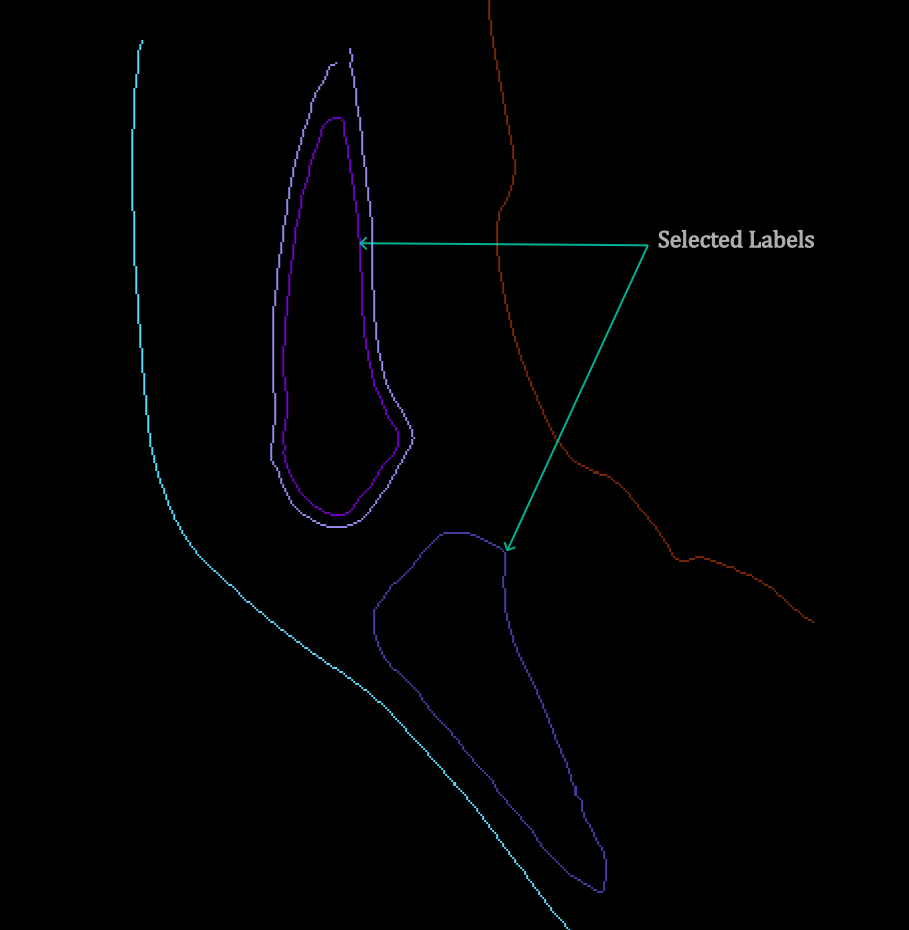
\includegraphics[width=0.7\linewidth]{label_selected}
	\caption{Output from the labeling algorithm with the representative edges for femur (top) and tibia(bottom) highlighted. Distinct colors represent a different label identified by the labeling algorithm.}
	\label{fig:labelimg}
\end{figure}
 
After choosing the appropriate labels, a binary image for each frame is obtained, where the foreground has the boundary for the interior edge of tibia and femur, and the background has intensity value of zero.   

\textbf{Step 3: Obtaining the set of reference points}

After isolating the binary edge images of the tibia and femur in Step 2, the next task is to identify a set of reference points along these binary edges. Captured when the knee is fully flexed, this reference frame served as the baseline for further analysis, with transformations initially set to zero. The purpose of establishing these reference points is so that it ensures a consistent basis for accurately calculating the rigid transformations between subsequent frames. The direct use of the densely packed unordered binary edge data would be computationally cumbersome and less precise for such transformations.

To begin, the points along the boundary were organised in a systematic manner by sorting. This was done by first, defining a starting point, and then iteratively using a greedy nearest neighbor algorithm for sorting \parencite{Hinneburg2000neare-5849}. The most distal point of the bone was taken as the initial seed. Afterwards, the algorithm then selects the nearest neighboring point as the next point in the sequence. It continues to do this iteratively—choosing the closest point that hasn't been selected yet—until all points are sorted in a path that follows the boundary of the bone.

Once the points were sorted, the next step involved downsampling these points to a set of uniform equidistant reference points along the boundary of the binary edge. Directly sampling every n-th point from the sorted list did not suffice, as it resulted in uneven spacing due to the variable distances between consecutive points in the original boolean data.

The first step in this process was calculating the cumulative distances between each consecutive pair of points in the sorted list. Using these distances, a total path length was established. The desired interval between the new points was then determined by dividing this total path length by the number of intervals (number of desired points minus one). 

Determining the optimal number of points—ranging between 50 to 80—was established through trial and error. Fewer than 50 points often compromised the accuracy of the edge overlap by failing to capture the essential contours of the bone. Conversely, exceeding 80 points did not significantly enhance the algorithm's accuracy but increased the computation time slightly. 

To ensure that the position of points adhere closely to the original curve, yet remain equidistant, the cubic spline interpolation from SciPy's interpolate library was used. This routine used interpolation to add place points based on the above criteria. 
Figure \ref{fig:downsampled} depicts this result. 
\begin{figure}[H]
	\centering
	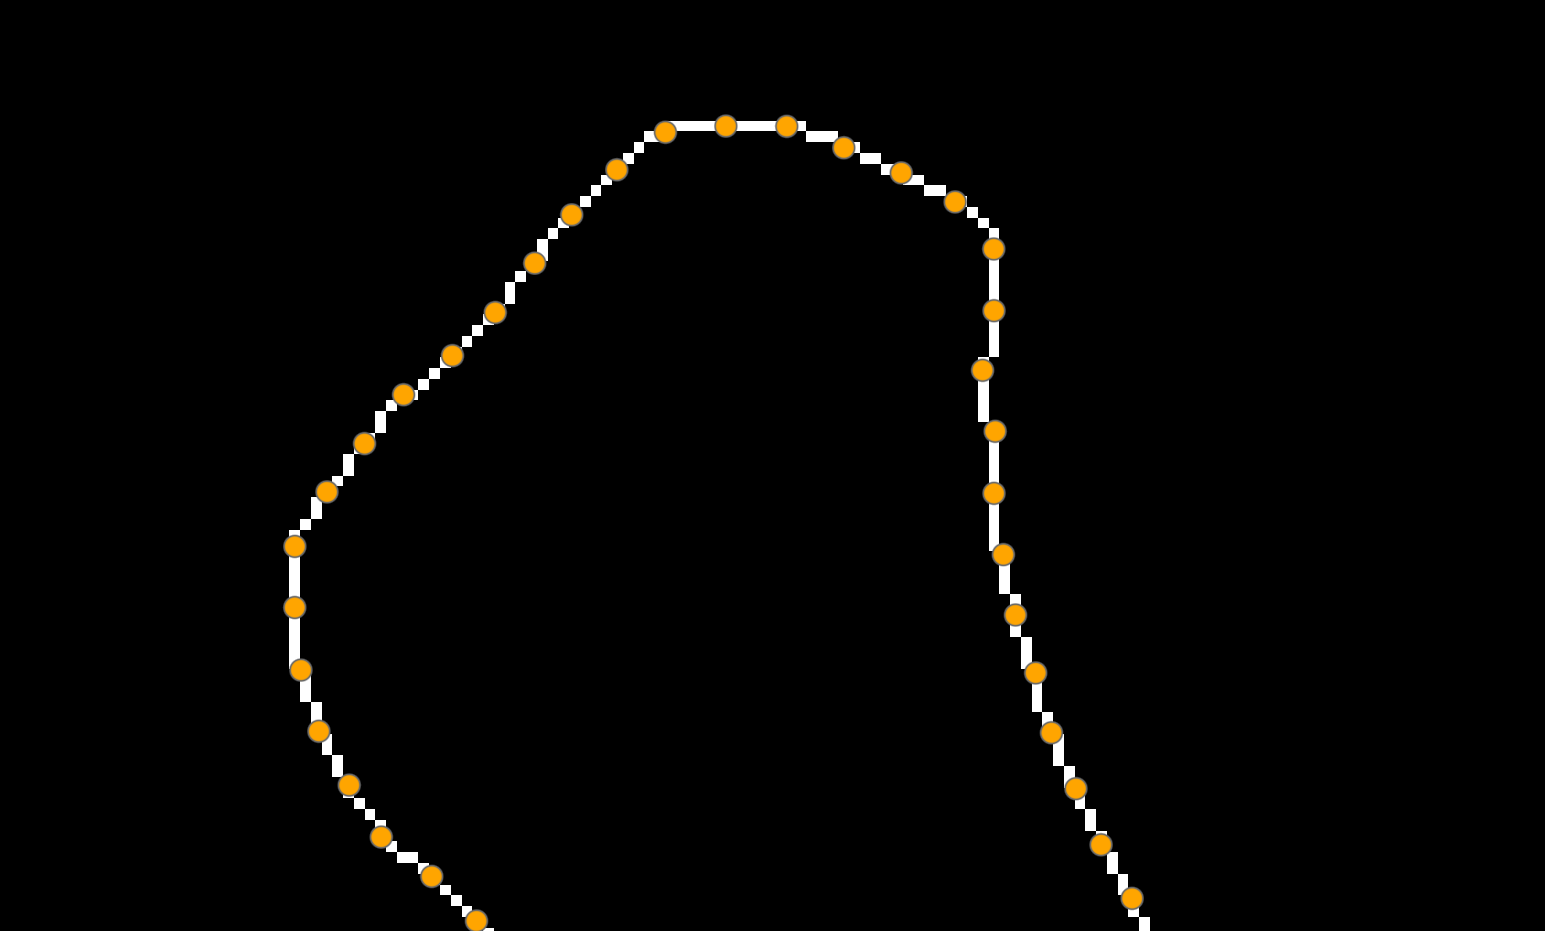
\includegraphics[width=0.7\linewidth]{downsampled}
	\caption{A close-up view at the equidistant sampled points (orange) along the boundary of the tibia edge (white) after completion of the sorting and downsample routine. }
	\label{fig:downsampled}
\end{figure}

\textbf{Step 4: Transformation matrices computation}

In this step, a set of transformation matrices was obtained, each containing the parameters that aligned the reference points from one frame to the next. These transformations included solely the translation in the sagittal plane and rotation about the transverse axis. This approach assumed that the bone does not undergo any deformation and that through-plane motion is negligible throughout the motion cycle. 

Mathematically, the transformation of each point from one frame to the next can be expressed as 
\begin{equation}
	\mathbf{p'} = \mathbf{R}(\phi) \mathbf{p} + \mathbf{t}
	\label{eq:rot} 
\end{equation}
where: 
\begin{itemize}
	\item $\mathbf{p}$ is the position vector of the point in its current frame
	\item $\mathbf{p'}$ is the position vector of the point after transformation
	\item $\phi$ is the angle of rotation
	\item $\mathbf{R}(\phi)$  is the rotation matrix, given by 
	 \[
	 \mathbf{R}(\phi) = 
	 \begin{bmatrix}
	 	\cos \phi & -\sin \phi \\
	 	\sin \phi & \cos \phi
	 \end{bmatrix}
	 \]
	 
	 \item $\mathbf{t}$ is the translation vector,
	 	\[
	 	t = \begin{bmatrix}
	 		\Delta x \\
	 		\Delta y
	 	\end{bmatrix}
	 	\]
 	\item $\Delta x$ and $\Delta y$ are the translations in the Cartesian coordinate system. 
\end{itemize}   
As such, only three parameters, $x$, $y$, and $\phi$ needed to be computed. To determine these parameters, a cost function was defined. This function, denoted as $C(x,y,\phi)$, quantifies the alignment error by calculating the 'cost' of deviations for any given set of transformation parameters. The minimization of this cost identifies the combination of parameters that achieves the best alignment or overlap of the transformed frame with the reference frame. A lower value of the cost function output indicates a closer match to the target frame, suggesting a better alignment, whereas a higher value signifies a less accurate alignment. The equation of the cost function is given in Equation \ref{eq:cost_func}:  
\begin{equation}
	C(\Delta x, \Delta y, \phi) = \sum_{p=1}^{N} \min_{q \in Q} \left( \sqrt{(x_q - x_p')^2 + (y_q - y_p')^2} \right)
	\label{eq:cost_func}
\end{equation}
where:
\begin{itemize}
	\item $ (x_p, y_p) $ are the coordinates of the points in the reference frame
	\item $(x_p', y_p')$ are the coordinates of points after being transformed:
	\begin{align*}
		x_p' &= \Delta x + x_p \cos(\phi) - y_p \sin(\phi) \\
		y_p' &= \Delta y + x_p \sin(\phi) + y_p \cos(\phi)
	\end{align*}
	\item $(x_q, y_q)$ are the coordinates of points in the target frame.
	\item $N$ is the number of points in the reference frame, and $Q$ represents all points in the target frame.
\end{itemize}

This cost function evaluates the alignment of transformed coordinates to target coordinates by calculating the sum of the shortest distances from each point in the transformed frame to the closest point in the target frame. Each $(x_p', y_p')$ is the position of a point from the reference frame after being transformed by the parameters $\Delta x$, $\Delta y$, and $\phi$. For each transformed point,the distance to every point $(x_q, y_q)$ in the target frame is computed, the minimum of these distances is selected, and sum these minimum distances across all points is calculated. This sum is the output of the cost function, which is optimized in the following step. 

The optimization of this cost function was performed using a nonlinear least squares approach where the initial guess of [0,0,0] was provided. This guess represented the starting point for the transformation parameters $\Delta x$, $\Delta y$ and $\phi$. The \texttt{fmin} function from SciPy’s optimization module was used for this purpose, which uses the Nelder-Mead simplex method \parencite{nelder_simplex_1965}. The algorithm was used with a function and parameter tolerance of $1 \times 10^{-8}$, and maximum iterations of 1000. This method iteratively explores the parameter space to find the set of parameters that result in the lowest cost function value. The optimization procedure continues until the change in the cost function is less than the specified tolerance or the maximum number of iterations is reached, indicating convergence to an optimal solution. Figure \ref{fig:edge_tracking} provides a visual representation of the overlap of the reference points from the fully flexed initial position to the frame where the lower leg has been rotated by an angle of 12 degrees as reported by the rotary angle encoder. 
\begin{figure}[H]
	\centering
	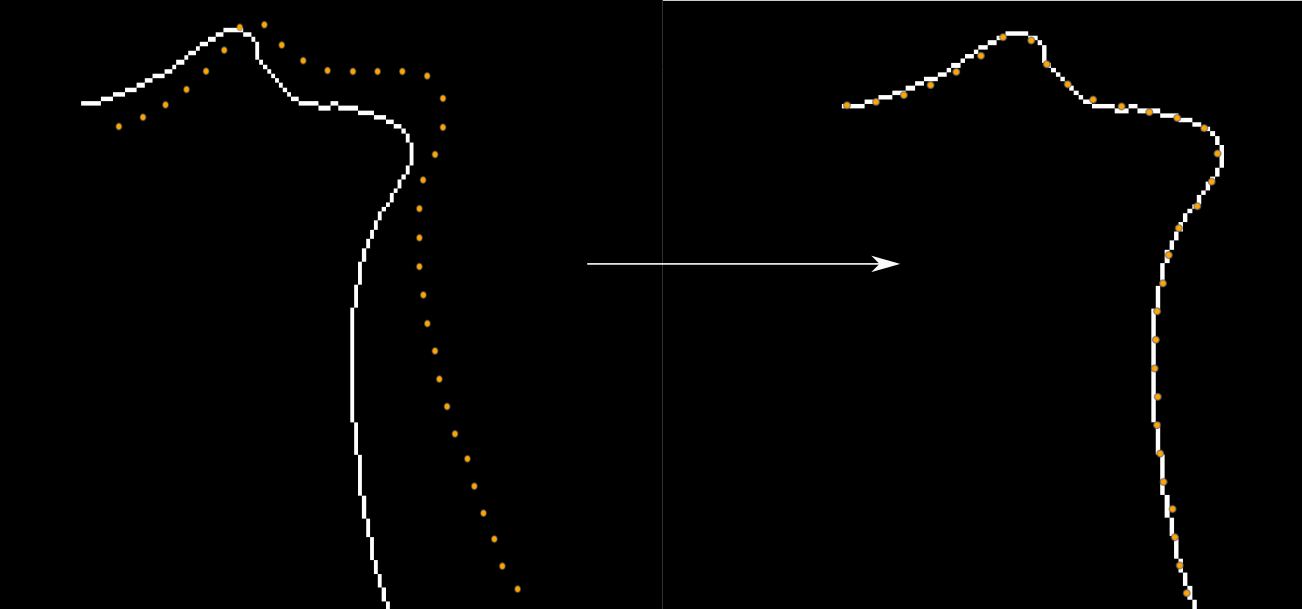
\includegraphics[width=0.7\linewidth]{image137}
	\caption{Left: The reference points in the first frame (orange) overlaid with the binary edge image of the target frame (white). Right: The reference points have been transformed by using the results from the optimization showing almost perfect overlap, illustrating the effective alignment achieved through the minimization of the cost function.}
	\label{fig:edge_tracking}
\end{figure}

These transformation matrices were obtained iteratively, where each set of transformed reference points served as the basis for the next iteration. Ultimately, a list of these matrices were obtained, containing information for each adjacent frame. 


\textbf{Step 5: Application of transformation matrices }

Given the transformation matrices obtained from edge tracking, any shape drawn on the first frame could now be transformed across the subsequent frames. If the initial edge detection covers the entire boundary of the bone, no further manual input is required, and the segmentation process is considered complete. However, for datasets where only a partial chunk of the full interior boundary of the bone (generally for the tibia) was found by edge detection, manual segmentation was necessary. This is illustrated in Figure \ref{fig:manualsegment}, which shows the tibia's boundary extended manually to complete the segmentation. 

\begin{figure} [H]
	\centering
	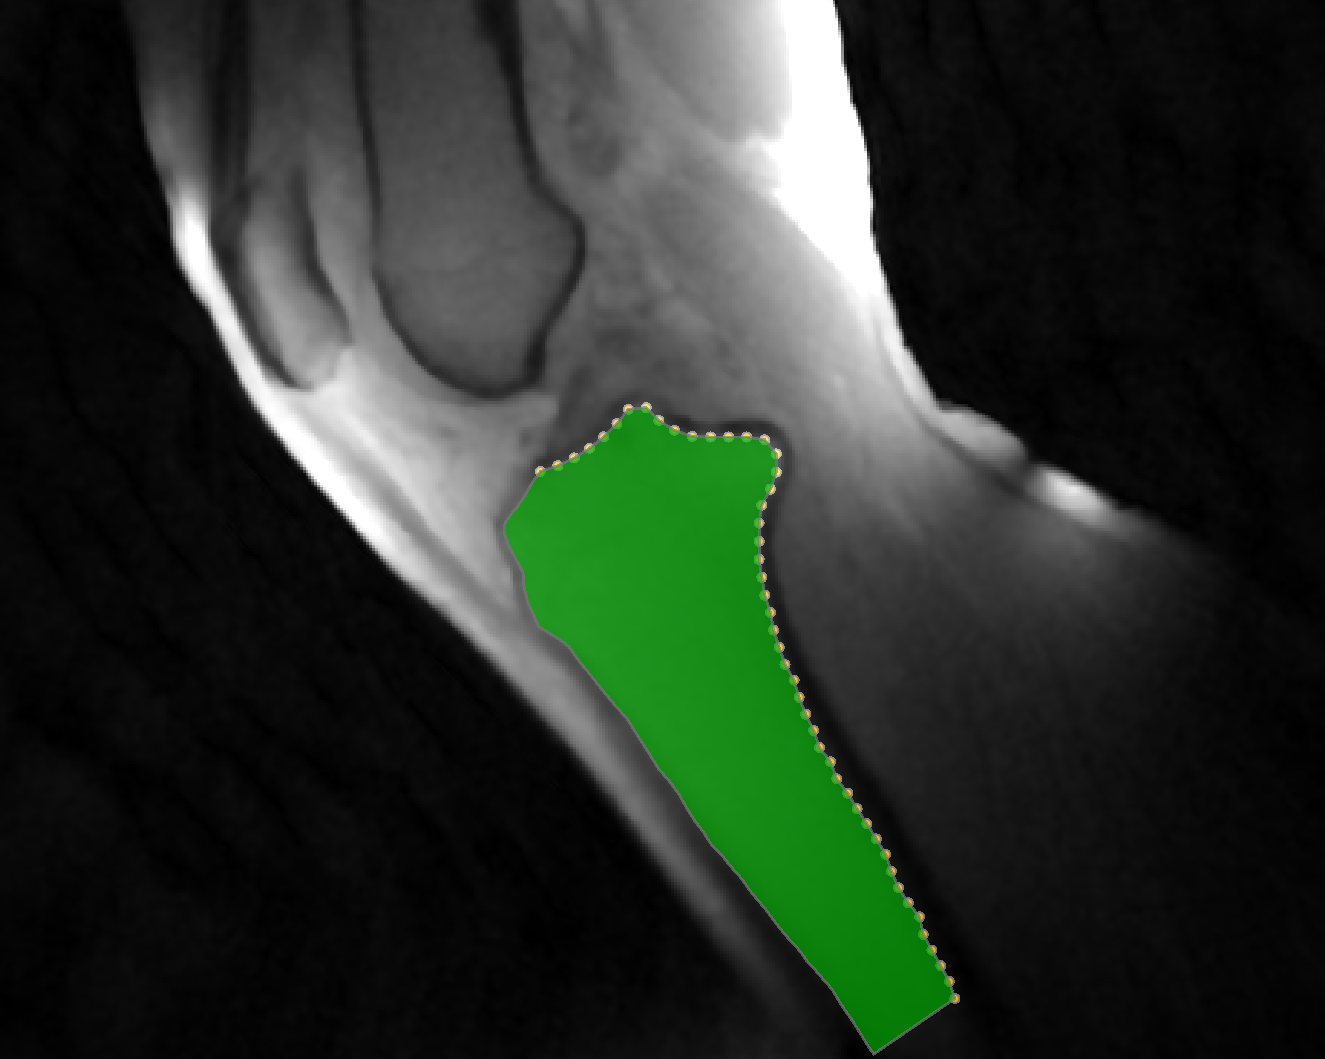
\includegraphics[width=0.7\linewidth]{manual_segment}
	\caption{Manual segmentation is performed to complete the boundary of the tibia's interior edge shown in green, along with the reference points (orange).}
	\label{fig:manualsegment}
\end{figure}

Using the shapes of these manually drawn segments, the transformation matrices were then applied to perform automatic segmentation in all subsequent frames. 

\textbf{Evaluation of Edge tracking algorithm}

To evaluate the accuracy of edge tracking achieved through cost function minimization, the deviation of the overlap between points on the transformed frame and the target frame was measured. 

The mean alignment error per point was derived by dividing the cost function output by the total number of points in the transformed frame. This value quantifies the average distance that a point on the transformed frame deviated from its corresponding point on the target frame. This value was calculated for all frames, and the average across all points and frames was taken for each dataset.

To assess the variability of these mean alignment errors across different datasets, the Standard Error of the Mean (SEM) was calculated using the following formula:
\begin{equation}
	\text{SEM} = \frac{\sigma}{\sqrt{n}}
\end{equation}
where $\sigma$ is the standard deviation of the mean alignment errors within each dataset, and $n$ is the number of frames analyzed per dataset.

\subsubsection{Extraction of Biomechanical Parameters}
After achieving automated segmentation of the tibia and femur across all frames, the next step involved extracting biomechanical parameters from the segmented regions. Two key metrics were considered for analysis to assess the relationship between these bones throughout the flexion-extension cycle captured in the 2D CINE images.

The first metric involved calculating the angle between the long axis of femur and tibia segments. This measurement provided insight into how the relative orientation of the two bones changes over time.

The second metric measured the distance between specific anatomical landmarks on both the femur and tibia. Tracking this distance across the frames offered an understanding of how the spatial relationship between these two bones evolved during the motion cycle. 

\textbf{Angle between the bones}

To calculate the angle between the bones, the long axis of each bone segment was identified using Principal Component Analysis (PCA) \parencite{jolliffe_principal_2004}. The analysis was performed using the PCA implementation from the scikit-learn (v1.3.1) Python library, a module for machine learning built on top of SciPy.

PCA determines the direction of maximum variance in the data, which coincides with the longitudinal axis of the bone. To perform PCA, the coordinates of the segmented binary mask are used as input. First, the centroid of the shape is calculated. This centroid is then subtracted from each data point, effectively centering the data. As a result of this transformation, the mean of the centered data points is shifted to (0, 0), meaning that the average position of all the data points is now at the origin of the coordinate system. 

Next, the covariance matrix (\text{Cov}) is computed, a square matrix that gives an indication of how the data varies along each dimension and how different dimensions vary together. 

\begin{equation}
	\mathbf{Cov} = 
	\begin{bmatrix}
		\mathrm{Var}(X) & \mathrm{Cov}(X,Y) \\
		\mathrm{Cov}(Y,X) & \mathrm{Var}(Y)
	\end{bmatrix}
	\label{eq:cov}
\end{equation}

where:
\begin{itemize}
	\item \(\mathrm{Var}(X)\) is the variance of \(X\), given by:
	\[
	\mathrm{Var}(X) = \frac{1}{N-1} \sum_{p=1}^{N} (X_{p} - \bar{X})^2,
	\]
	where \(N\) is the number of points, \(X_{p}\) represents the \(p^{th}\) point in the \(X\) dimension, and \(\bar{X}\) is the mean value of all points in the \(X\) dimension. 
	\item \(\mathrm{Cov}(X,Y)\) is the covariance between dimensions \(X\) and \(Y\), defined as:
	\[
	\mathrm{Cov}(X,Y) = \frac{1}{N-1} \sum_{p=1}^{N} (X_{p} - \bar{X})(Y_{p} - \bar{Y}),
	\]
	where \(Y_{p}\) represents the \(p^{th}\) point in the \(Y\) dimension, and \(\bar{Y}\) is the mean value of all points in the \(Y\) dimension.
	
	\item \(\mathrm{Cov}(Y,X)\) and  \(\mathrm{Var}(Y)\) are equal to their counterparts because the covariance matrix is symmetric. 

\end{itemize}


When this covariance matrix is applied to a vector, the matrix transforms the vector such that it aligns with the direction of maximum variance in the dataset. Therefore, by computing the matrix's eigenvectors and eigenvalues, the vectors representing the direction of maximum variance is identified. The first principal component refers to the eigenvector associated with the largest eigenvalue. In figure \ref{fig:longaxes}, the longitudinal axis of femur and tibia are shown. 

\begin{figure}[H]
	\centering
	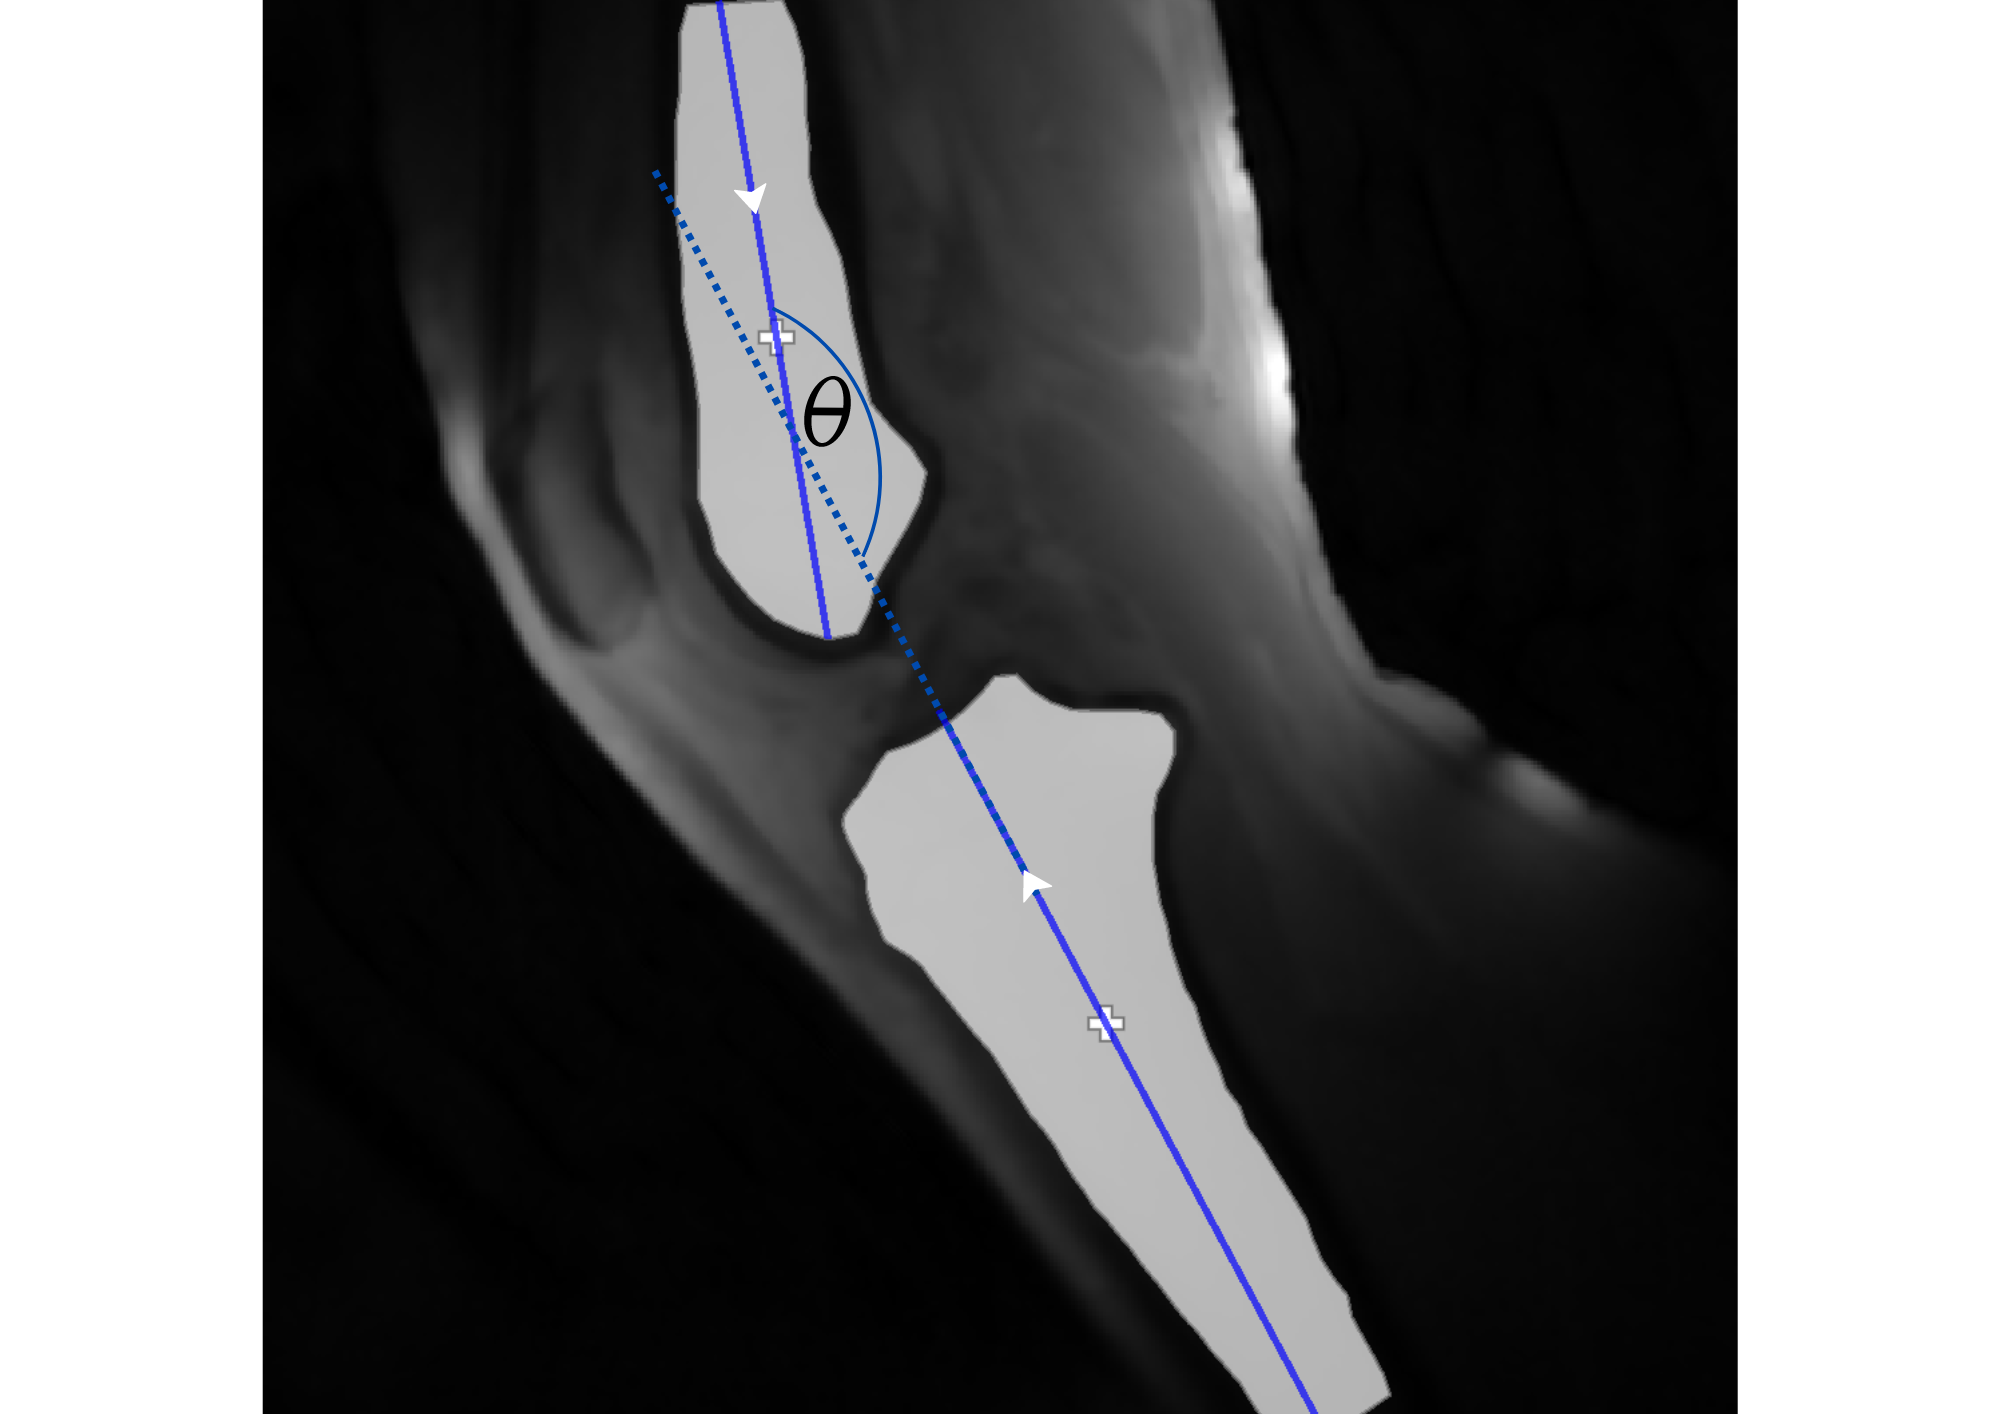
\includegraphics[width=0.7\linewidth]{theta_angle_new}
	\caption{The long axis of the bones are identified by using the PCA (blue) along with the centroid (white cross) for each segment. $\theta$ represents the obtuse angle between the vectors of the axes}
	\label{fig:longaxes}
\end{figure}

The angles between the segments was calculated by using the dot product between unit vectors:

\begin{equation}
	\theta = \arccos(\mathbf{U}_{\text{fem}} \cdot \mathbf{U}_{\text{tib}})
	\label{eq:angle}
\end{equation}
where, $\mathbf{U}_{\text{fem}}$ and $\mathbf{U}_{\text{tib}}$ are the unit vectors of the longitudinal axes for the femur and tibia segments respectively. The range of $\theta$, the angle between the femur and tibia, is from 0° to 180°. As the knee extends, this angle is increases up to 180°. Should it extend beyond this point, the excess is added rather than subtracted, allowing the visualization of angles exceeding 180°. 

\textbf{Distance between the bones}

To quantify the spatial relationship between the bones, anatomical landmarks on the femur and the tibia were chosen. For the femur, the most distal point on its segment was selected, and for the tibia, a  proximal point lying in the notch was chosen, as illustrated in Figure \ref{fig:twopoints}.   
\begin{figure}[H]
	\centering
	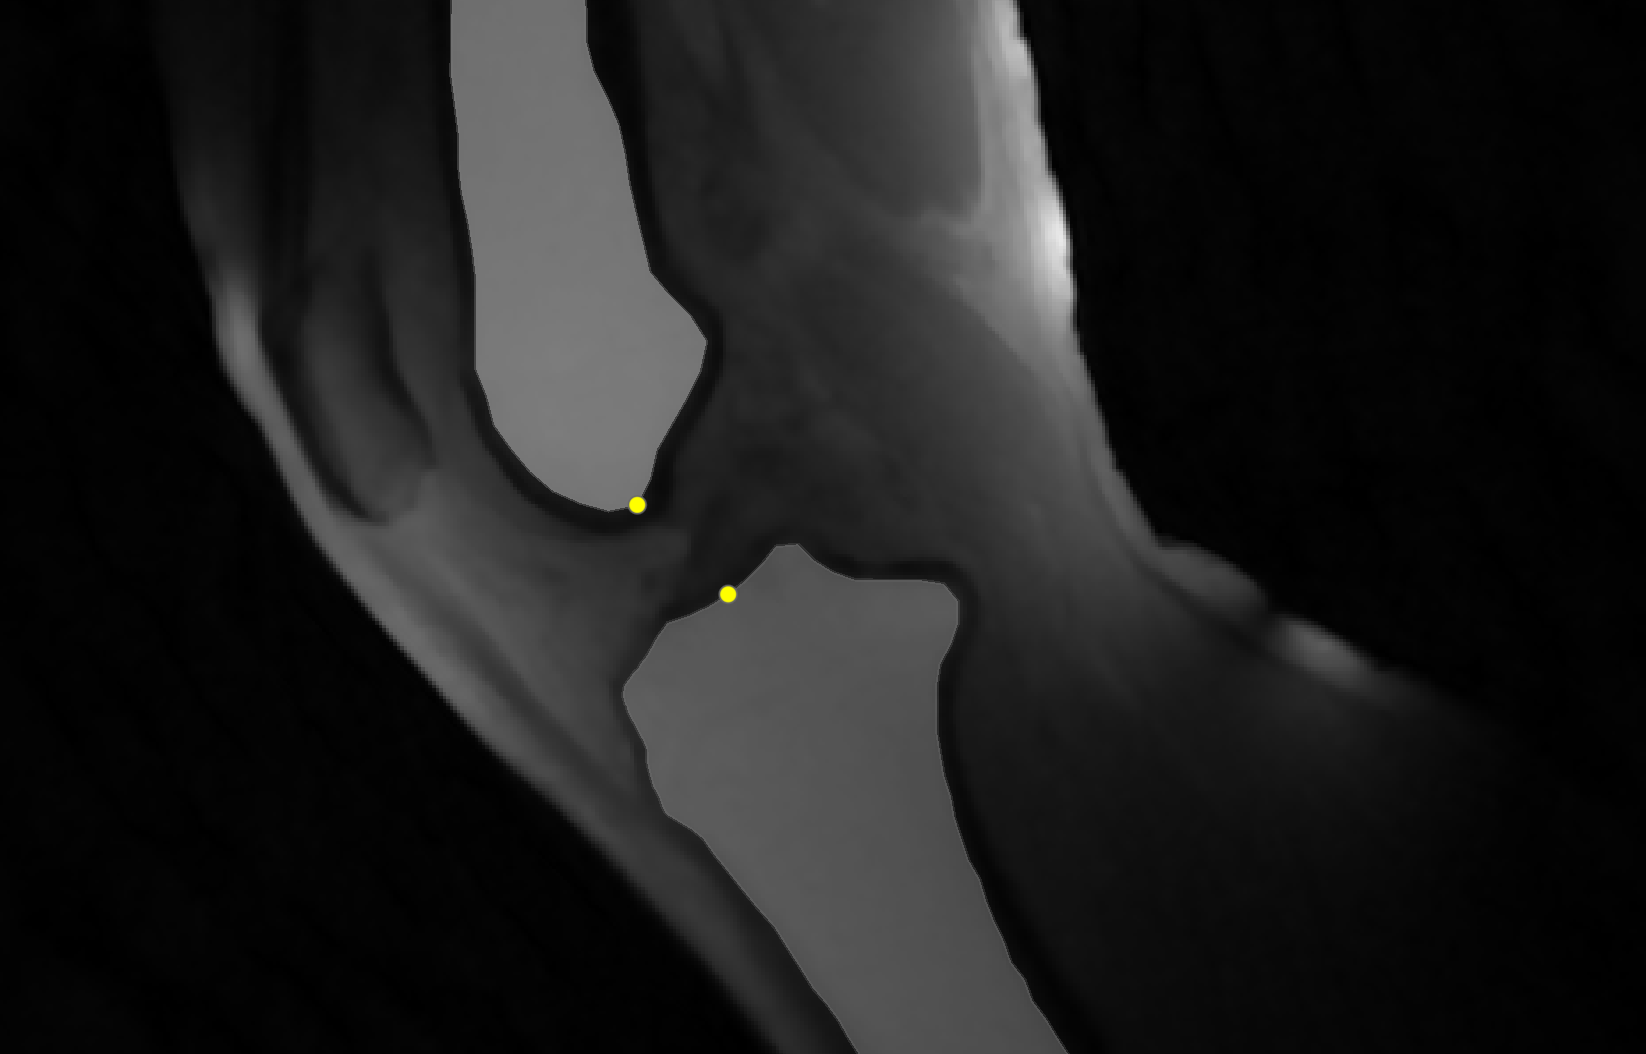
\includegraphics[width=0.7\linewidth]{two_points}
	\caption{Segmented femur and tibia displayed in solid gray, superimposed on the knee's MRI image at a specific point in the flexion cycle. The anatomical landmarks on the femur and tibia are marked in yellow}
	\label{fig:twopoints}
\end{figure}

These points were selected based on their consistent availability and reliable identification in the chosen MRI slices of each dataset.

The euclidean distance between the femur landmark ($y_2, x_2$) and the tibia landmark ($y_1, x_1$) was measured by using Equation \ref{eq:distance}. 
\begin{equation}
	d = \sqrt{(y_2 - y_1)^2 + (x_2 - x_1)^2}
	\label{eq:distance}
\end{equation} 


\textbf{Normalizing the x-axis for analysis and graphical purposes}

Even though the number of frames is consistent between the loaded and unloaded conditions for a given dataset, the total number of frames reconstructed varies across different datasets due to the varying ranges of motion achieved by the subjects inside the scanner during the experiment. 

The variation in frame count necessitated the normalization of the time axis across all datasets to ensure consistent analysis and comparison. The nature of the exercise is such that each dataset inherently begins at a maximally flexed position—where the leg touches the bore of the scanner—and extends to maximum, where the leg is parallel to the scanner bore, before flexing back to the original position. This movement cycle, from -100\% for maximal flexion, through 0\% at full extension, and back to +100\% for maximal flexion, was consistent across all datasets. To facilitate the comparison and aggregation of biomechanical parameters, the normalized time axis was divided into bins of 10 degrees. Data were aggregated within each bin across all datasets, and the center of each bin was selected as the plotting point for graphical representation

For statistical analysis, a two-sample independent t-test was performed for each bin using the \texttt{stats} module from the  SciPy library. This analysis was aimed at testing the null hypothesis that any observed differences in parameters under loaded and unloaded conditions could be attributed to random chance. 


\section{Results}
\label{sec:yetanother}

\subsection{Edge tracking and segmentation}

The measured alignment error per point for the femur and the tibia are presented separately in Figures \ref{fig:barfemur} and \ref{fig:bartibia} respectively. 
\begin{figure}[H]
	\centering
	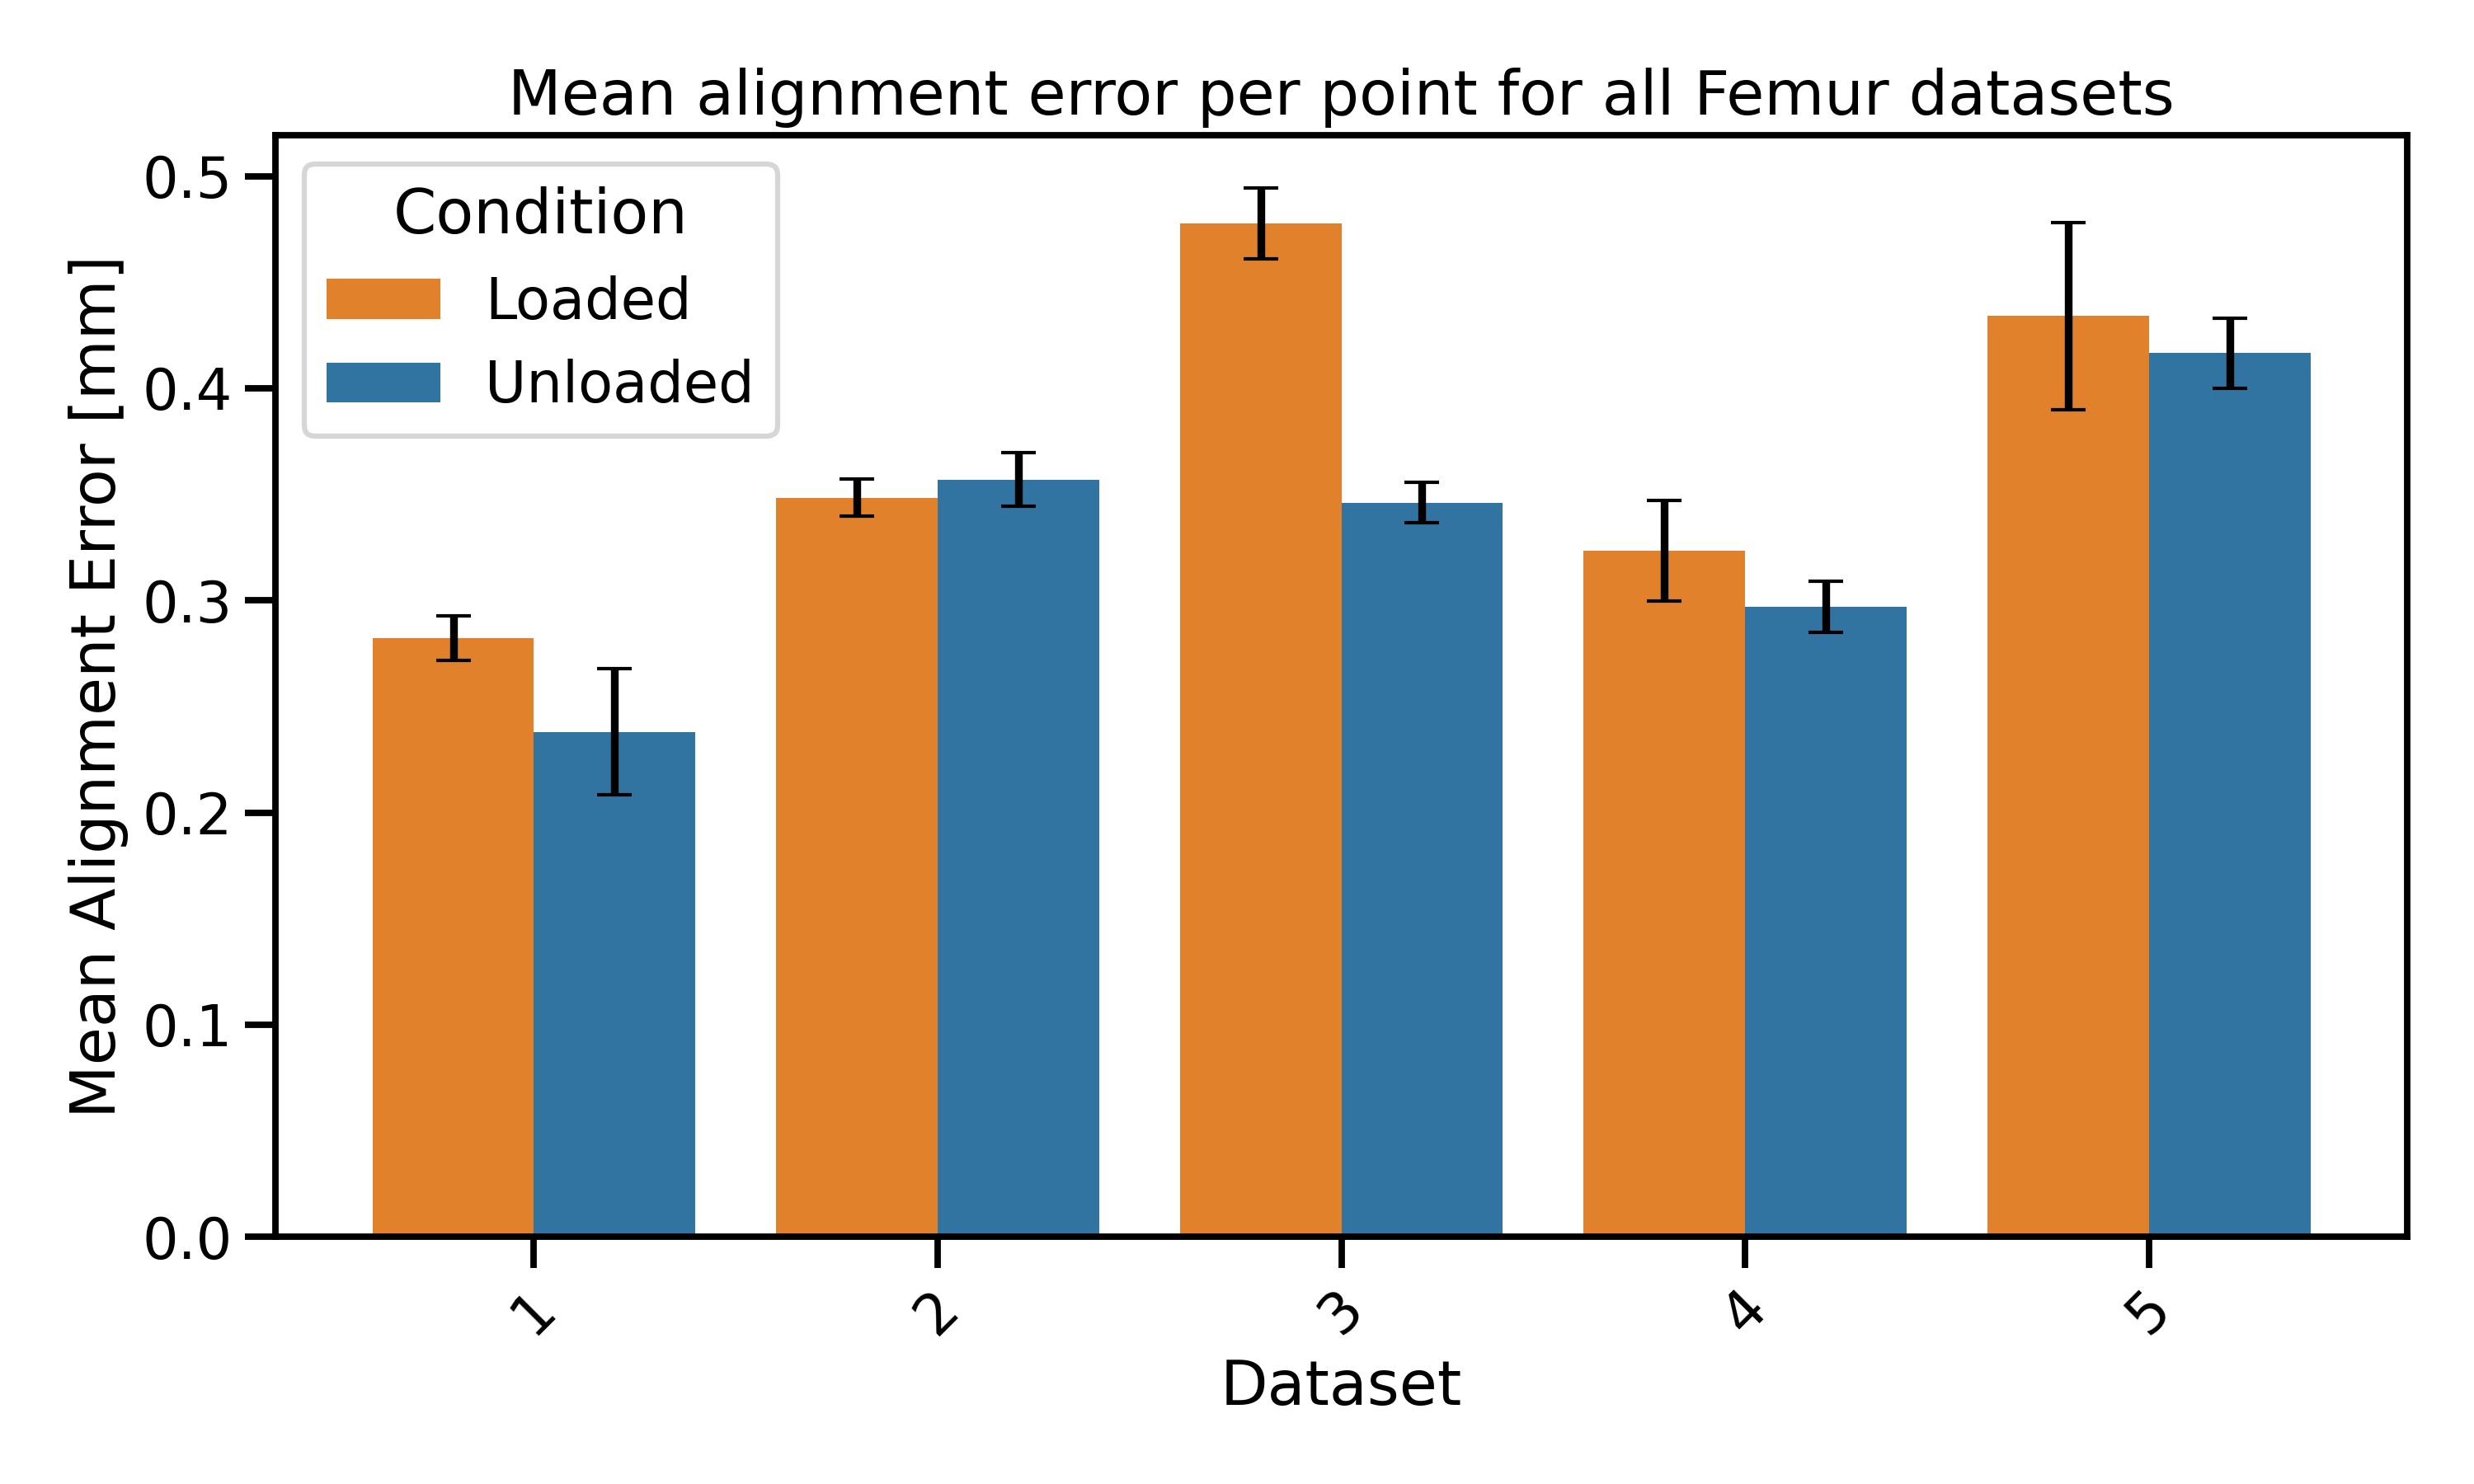
\includegraphics[width=0.7\linewidth]{bar_no_1_3_Femur_both.png}
	\caption{Bar chart illustrating the mean alignment error per point for edge tracking in femur datasets under loaded (orange) and unloaded (blue) conditions. Error bars represent the standard error of the mean (SEM) across frames for each condition within each dataset.}
	\label{fig:barfemur}
\end{figure}

\begin{figure}[H]
	\centering
	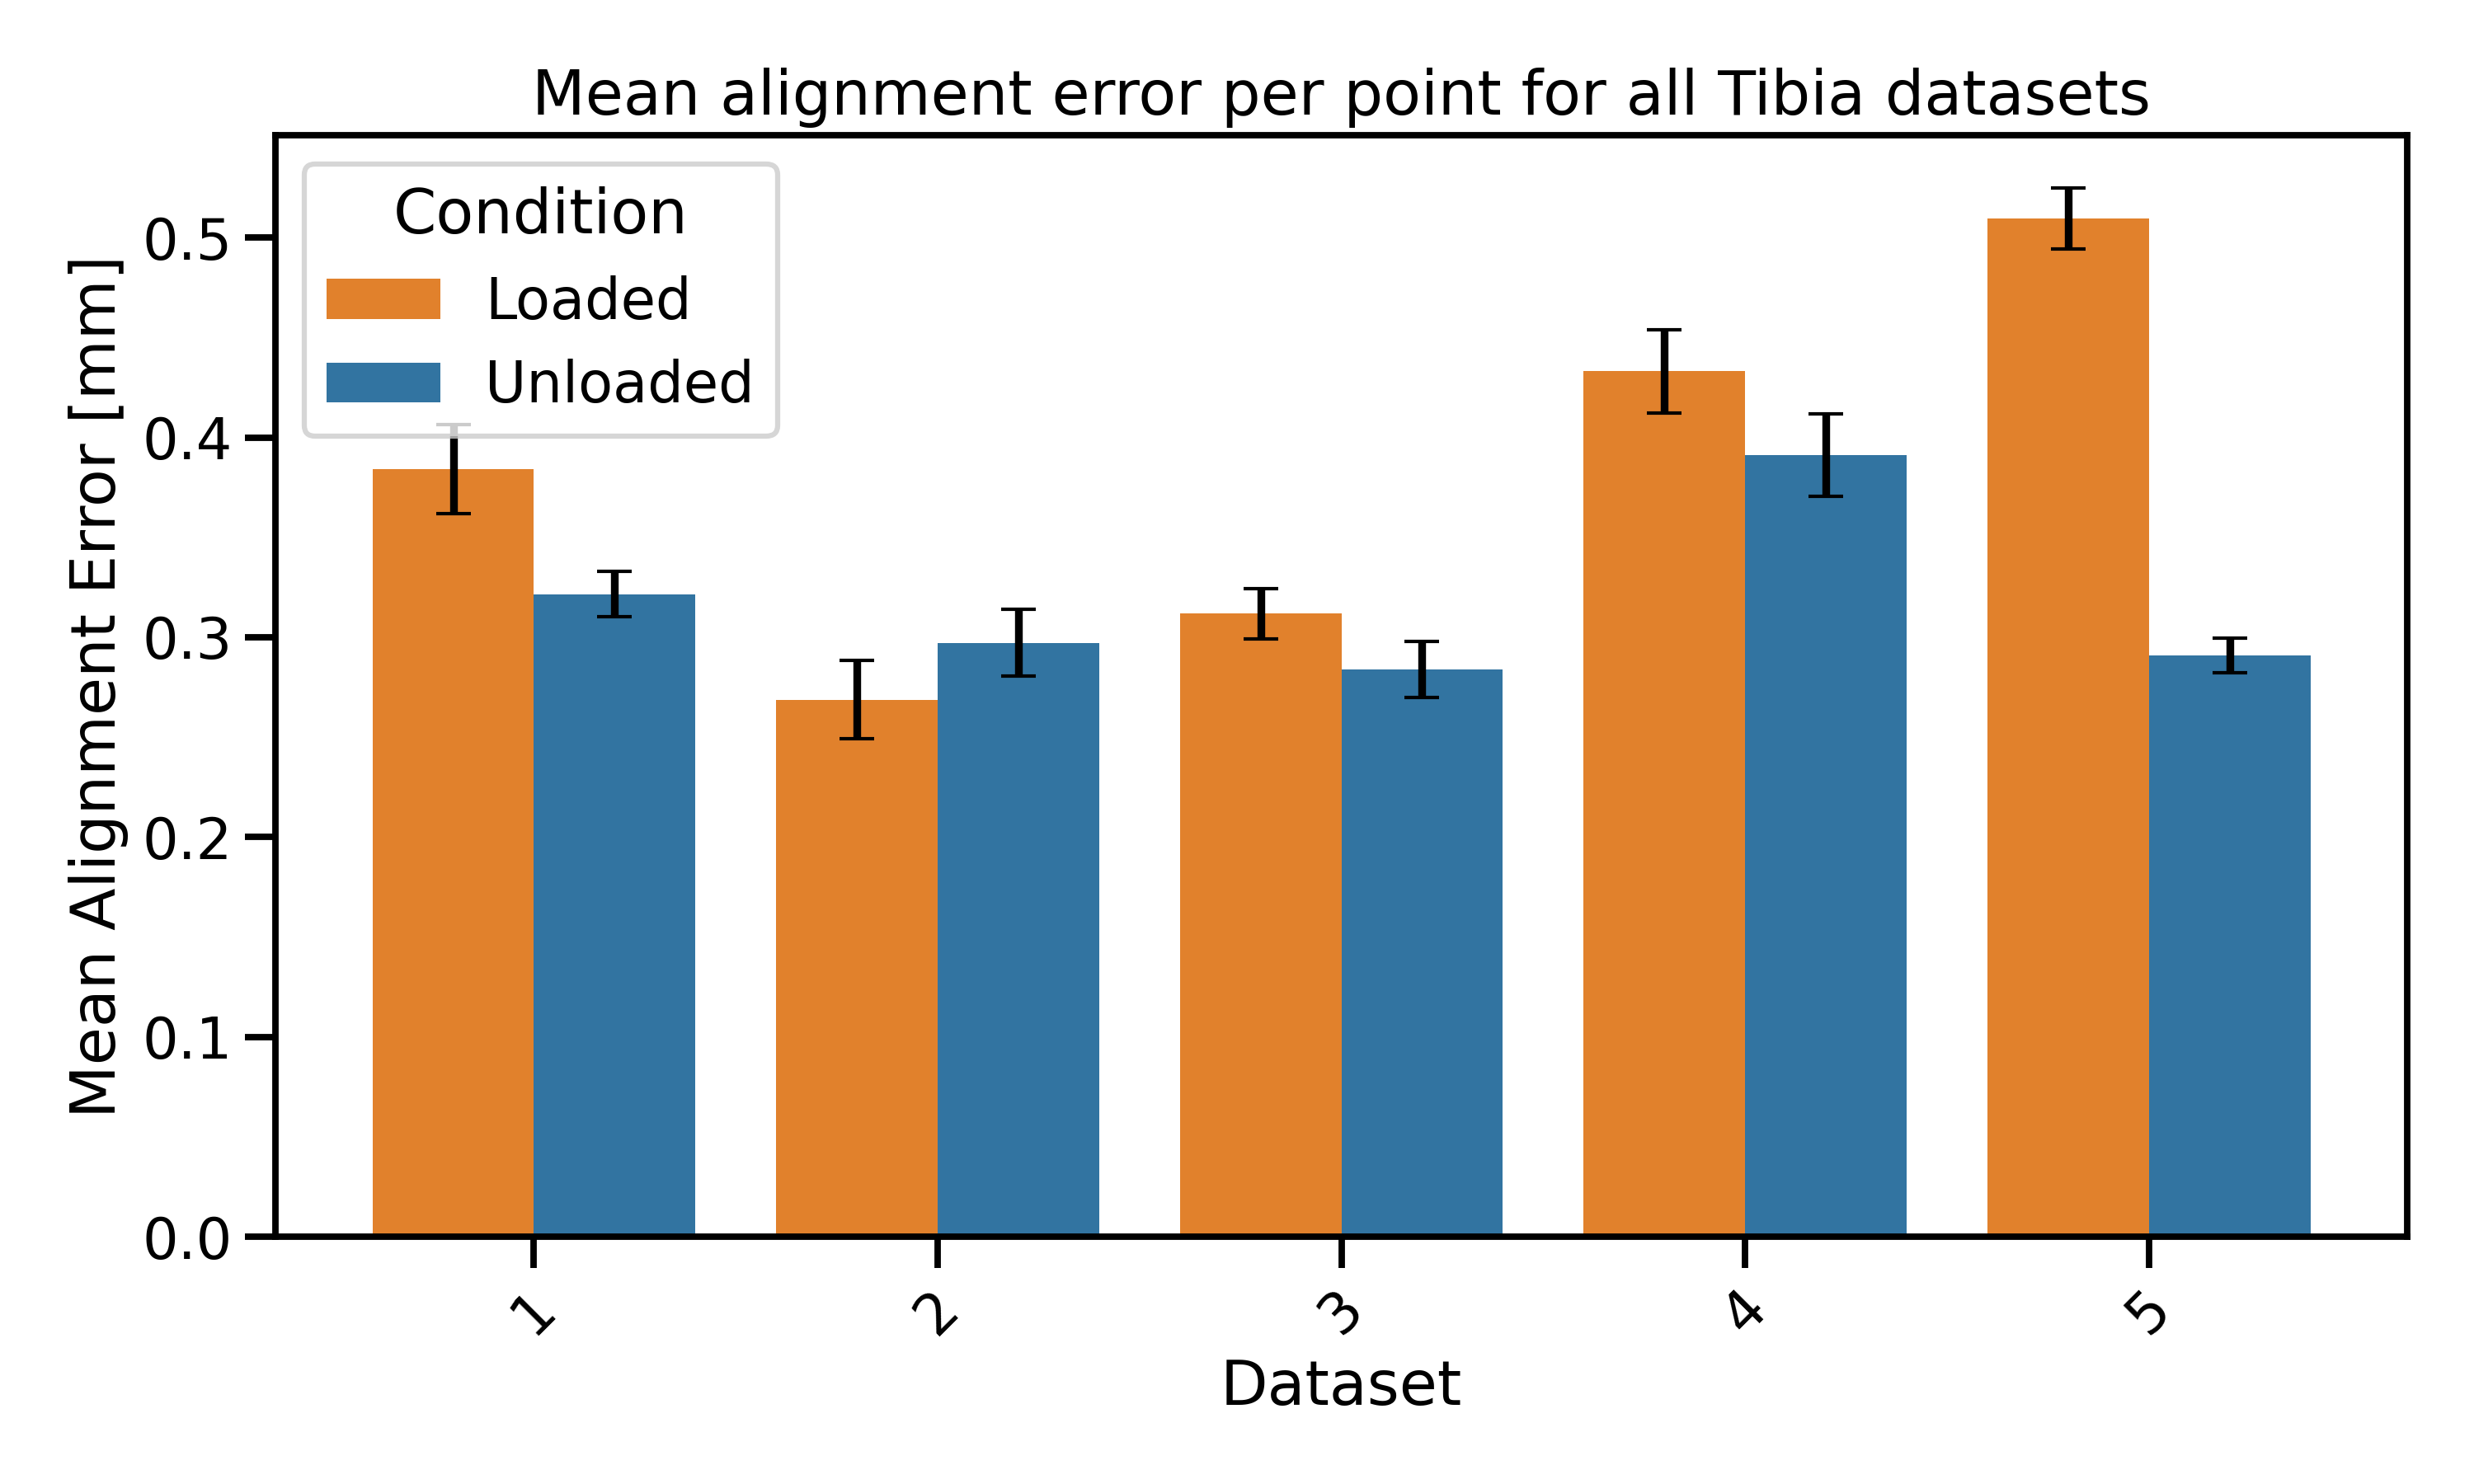
\includegraphics[width=0.7\linewidth]{bar_no_1_3_Tibia_both.png}
	\caption{Bar chart illustrating the mean alignment error per point for edge tracking in tibia datasets under loaded (orange) and unloaded (blue) conditions. Error bars represent the standard error of the mean (SEM) across frames for each condition within each dataset.}
	\label{fig:bartibia}
\end{figure}

A lower value of the y-axis in these bar charts indicates better accuracy of the edge tracking algorithm. Error bars reflect the standard error of the mean (SEM) for each condition within each dataset, demonstrating the precision of the mean alignment error estimates.  

For the femur datasets, The highest mean alignment error observed was 0.48 mm ± 0.04 mm, indicating that dataset 3 under load had the least precision in edge tracking. Conversely, the lowest mean alignment error was 0.24 mm ± 0.01 mm, suggesting that dataset 1 without load had the best edge tracking accuracy. On average, the mean alignment error for the loaded condition was 0.37 mm ± 0.02 mm, while for the unloaded condition, it was 0.33 mm ± 0.02 mm.

Similarly, for the tibia datasets, the highest mean alignment error observed was 0.51 mm ± 0.02 mm, implying that dataset 5 under load had the least precision in edge tracking for the tibia . Conversely, the lowest mean alignment error recorded was 0.27 mm ± 0.01 mm, suggesting that the edge tracking in tibia worked best for dataset 2 also under load. On average, the mean alignment error for the loaded condition was 0.38 mm ± 0.02 mm, while for the unloaded condition, it was 0.32 mm ± 0.01 mm.

A paired sample t-test was conducted to compare the mean alignment errors per point between the loaded and unloaded conditions across five datasets for the femur and tibia datasets. The null hypothesis tested was that there is no significant difference in the average values of mean alignment errors between the two conditions. The p-values obtained were 0.087 for the femur datasets and 0.057 for the tibia datasets. Given these p-values, the null hypothesis was not rejected for either dataset, suggesting no statistically significant difference in the mean alignment errors between the conditions at the conventional 0.05 significance level.
   
To illustrate how this alignment error translates to actual performance of the segmentation, the worst performing dataset, which is the loaded case for the femur for dataset 5 is shown in Figure \ref{fig:d5wfem}: 

\begin{figure}[H]
	\centering
	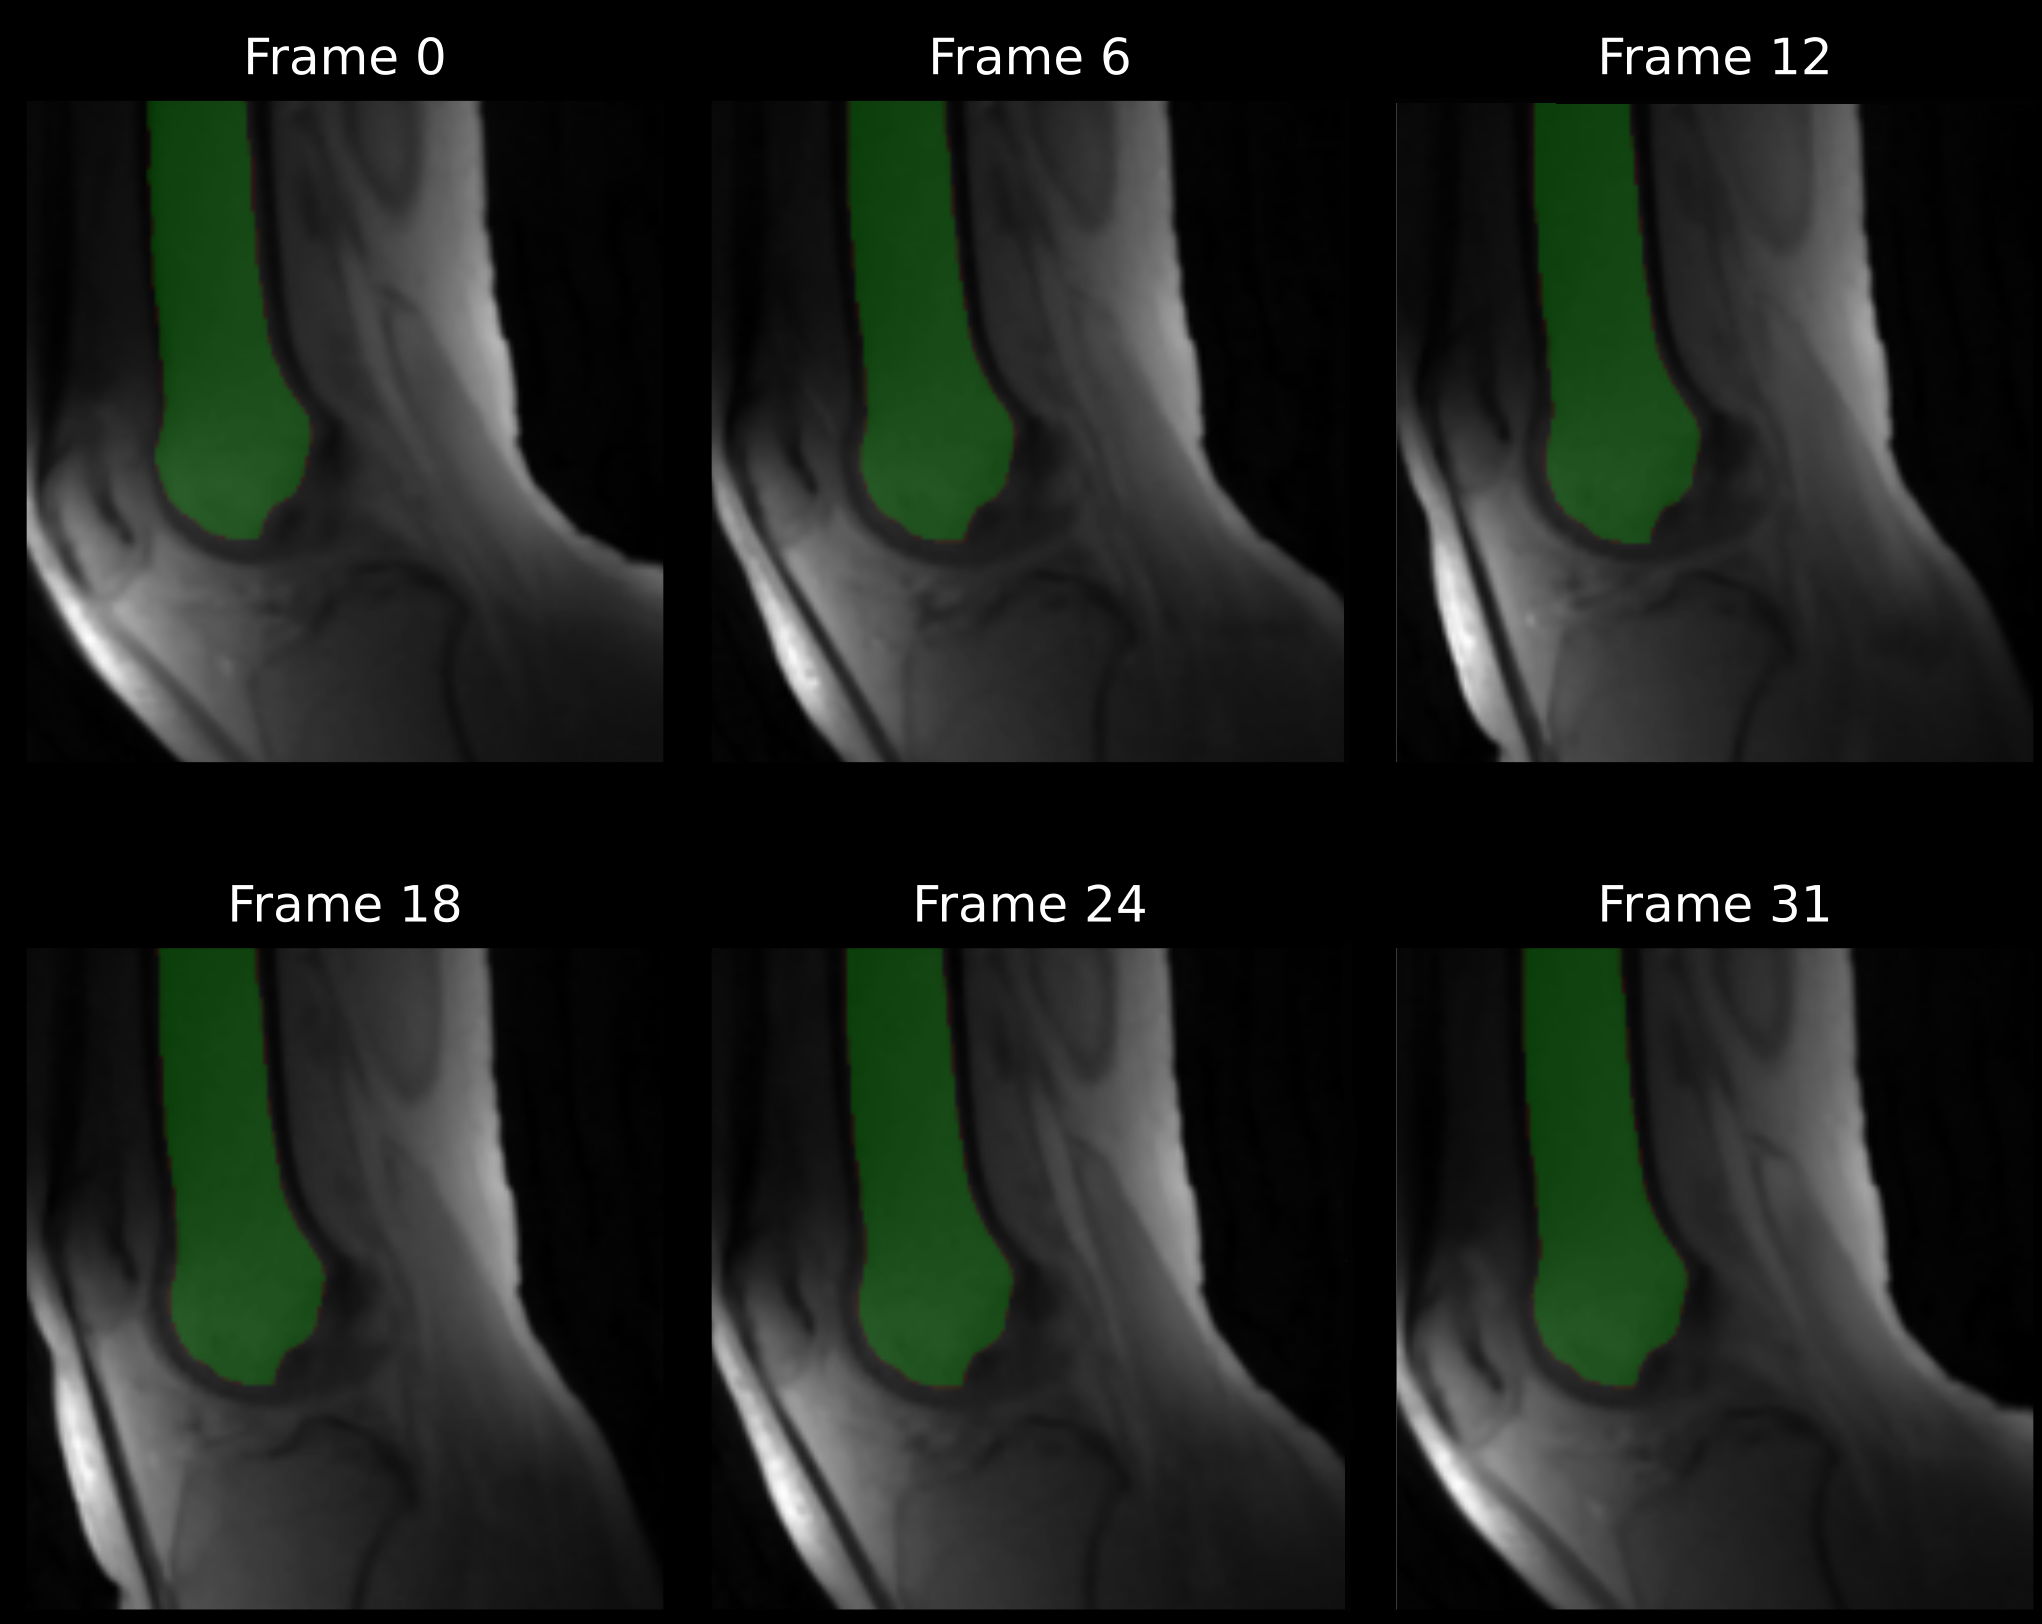
\includegraphics[width=0.7\linewidth]{d5_W_fem}
	\caption{ The result of the proposed automatic segmentation of the femur (shown in green) for dataset 3 under load at various time points during the extension-flexion cycle. Frame 0 and Frame 31 represent the knee at maximally flexed positions, at the start and end of the full cycle.}
	\label{fig:d5wfem}
\end{figure}

As for the tibia dataset, the worst performing dataset is illustrated similarly in Figure \ref{fig:d7wtib}. 

\begin{figure} [H]
	\centering
	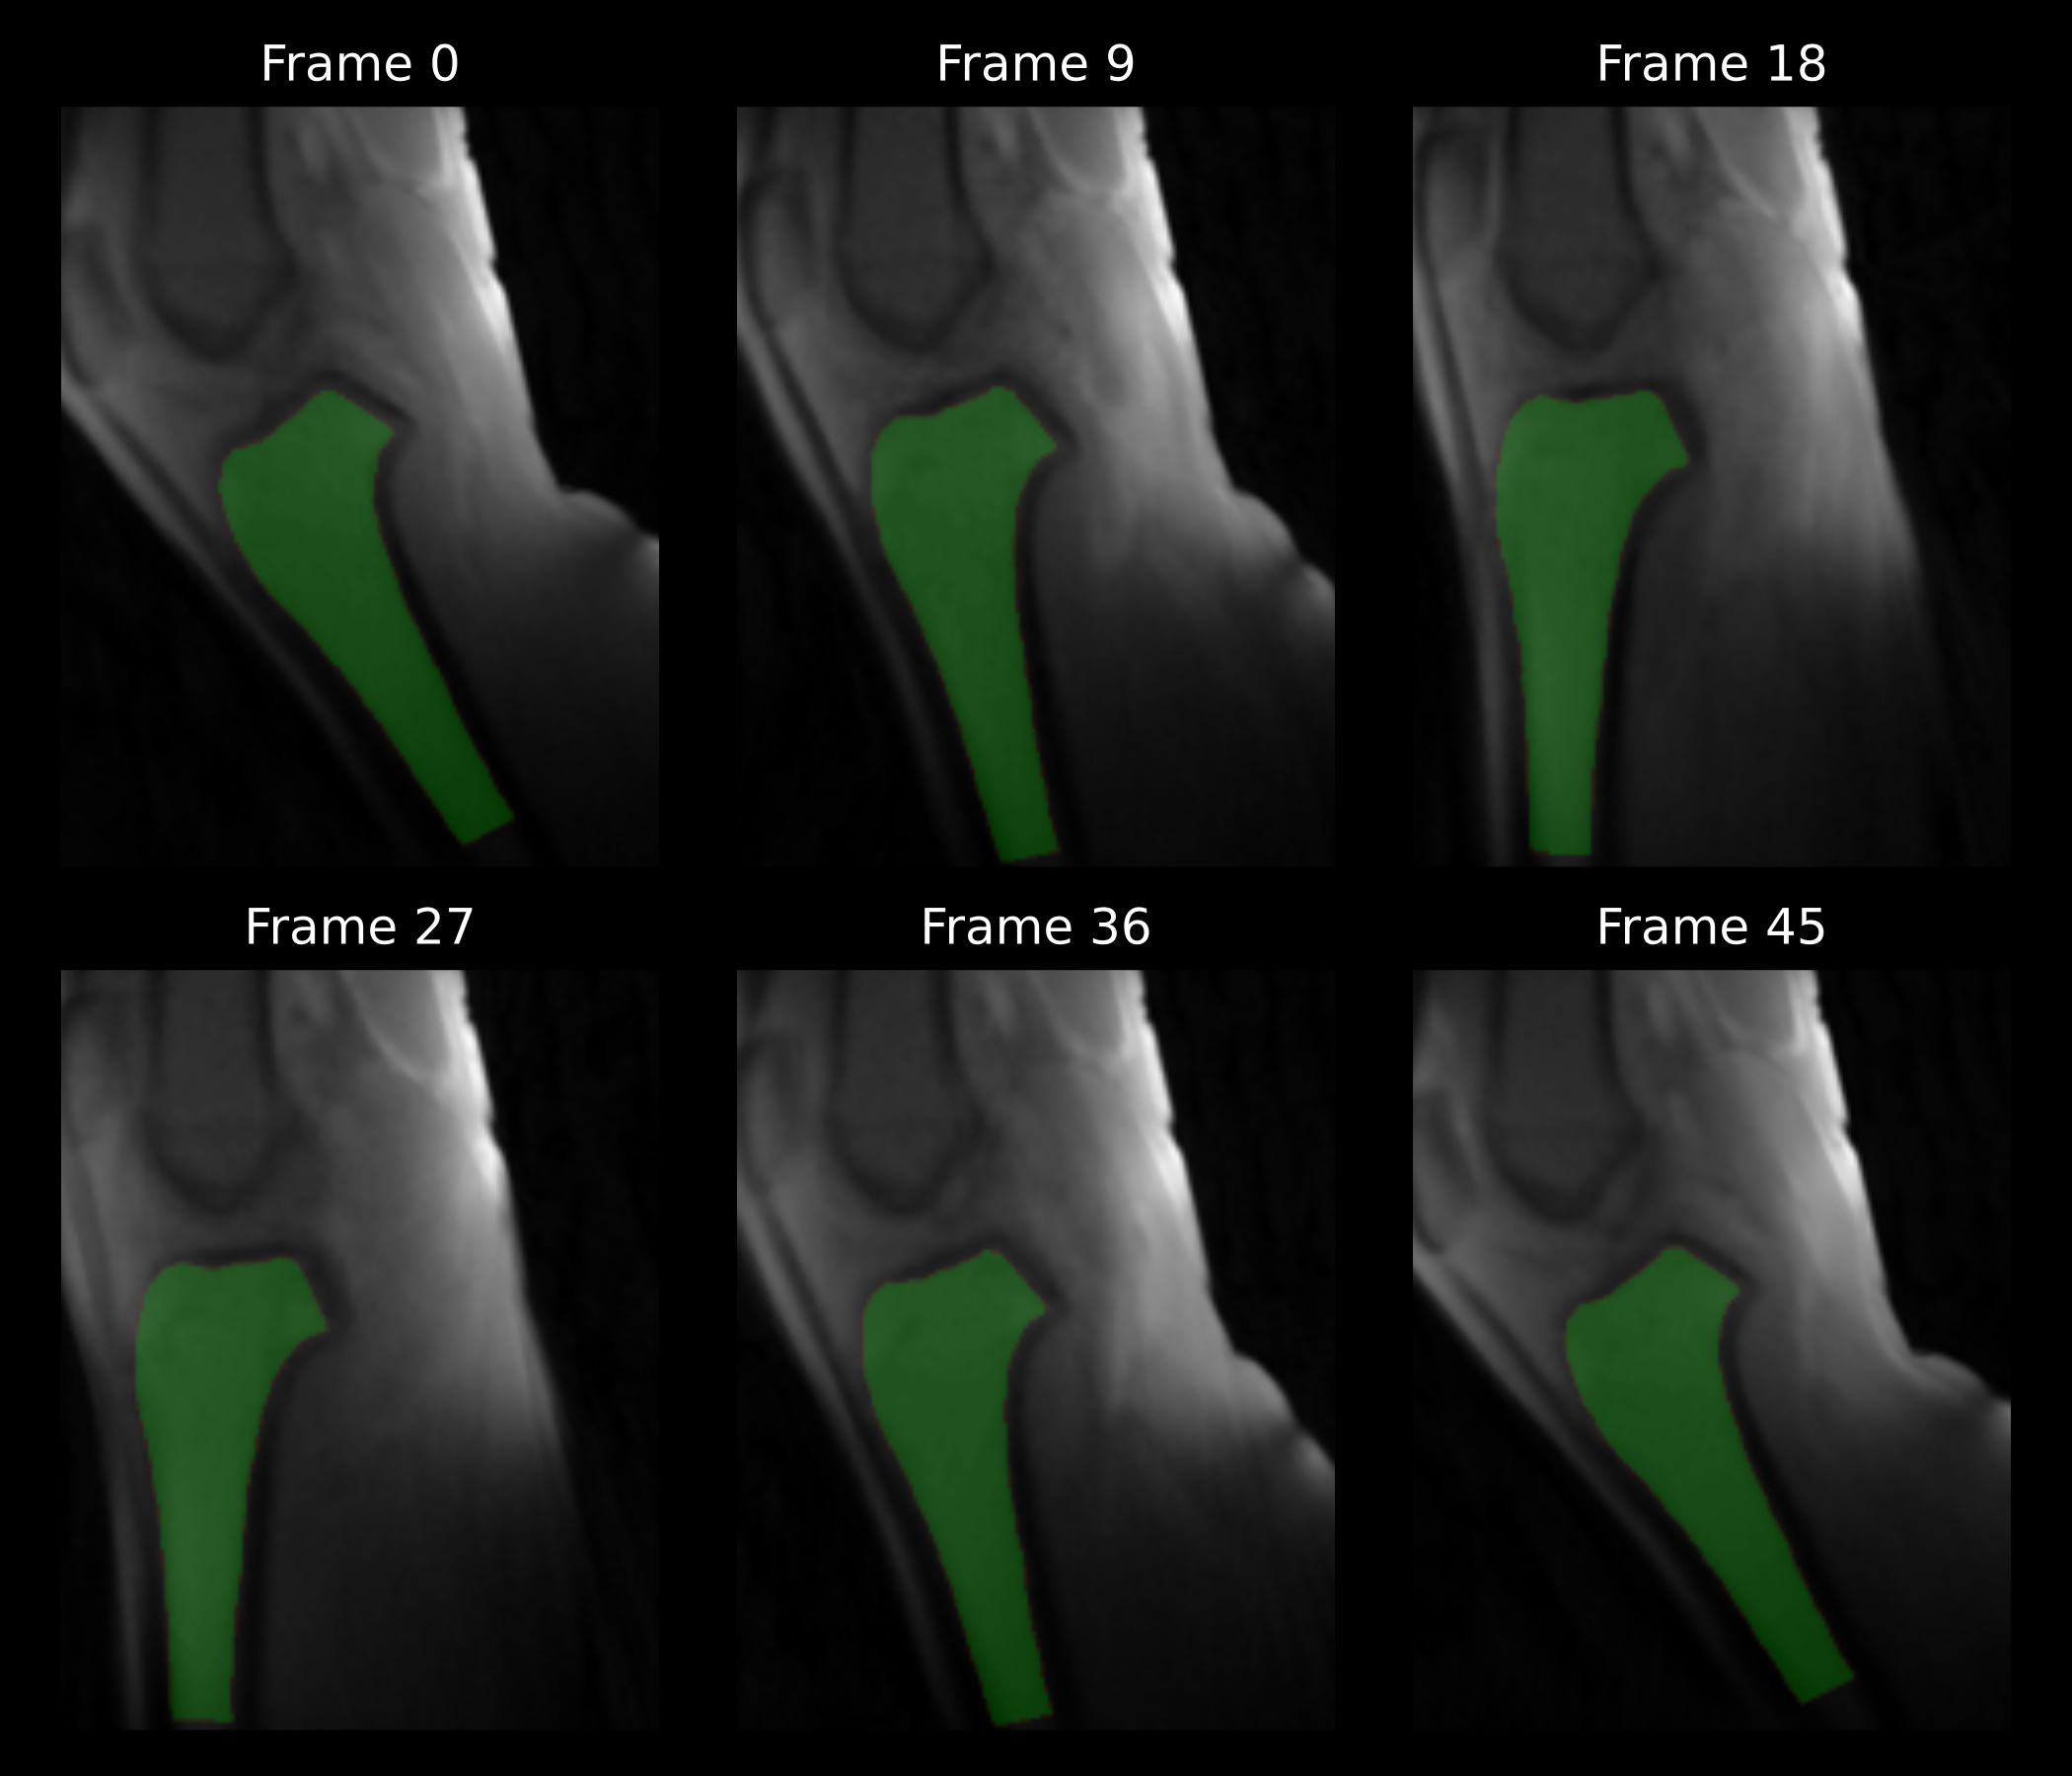
\includegraphics[width=0.7\linewidth]{d7_W_tib}
	\caption{ The result of automatic segmentation of the tibia (shown in green) for dataset 5 under load at various time points during the extension-flexion cycle. Frame 0 and Frame 45 represent the knee at maximally flexed positions, at the start and end of the full cycle respectively.}
	\label{fig:d7wtib}
\end{figure}
 
The results above demonstrate that despite the highest magnitude of mean alignment error per point, the error is not visually perceptible in the segmentation.   

\subsection{Biomechanical parameter extraction}

\textbf{Angle calculation}

Figure \ref{fig:anglegraphstickman} displays the result of calculating the angle between the long axes of bone segments across the flexion-extension cycle. 
 
\begin{figure}[H]
	\centering
	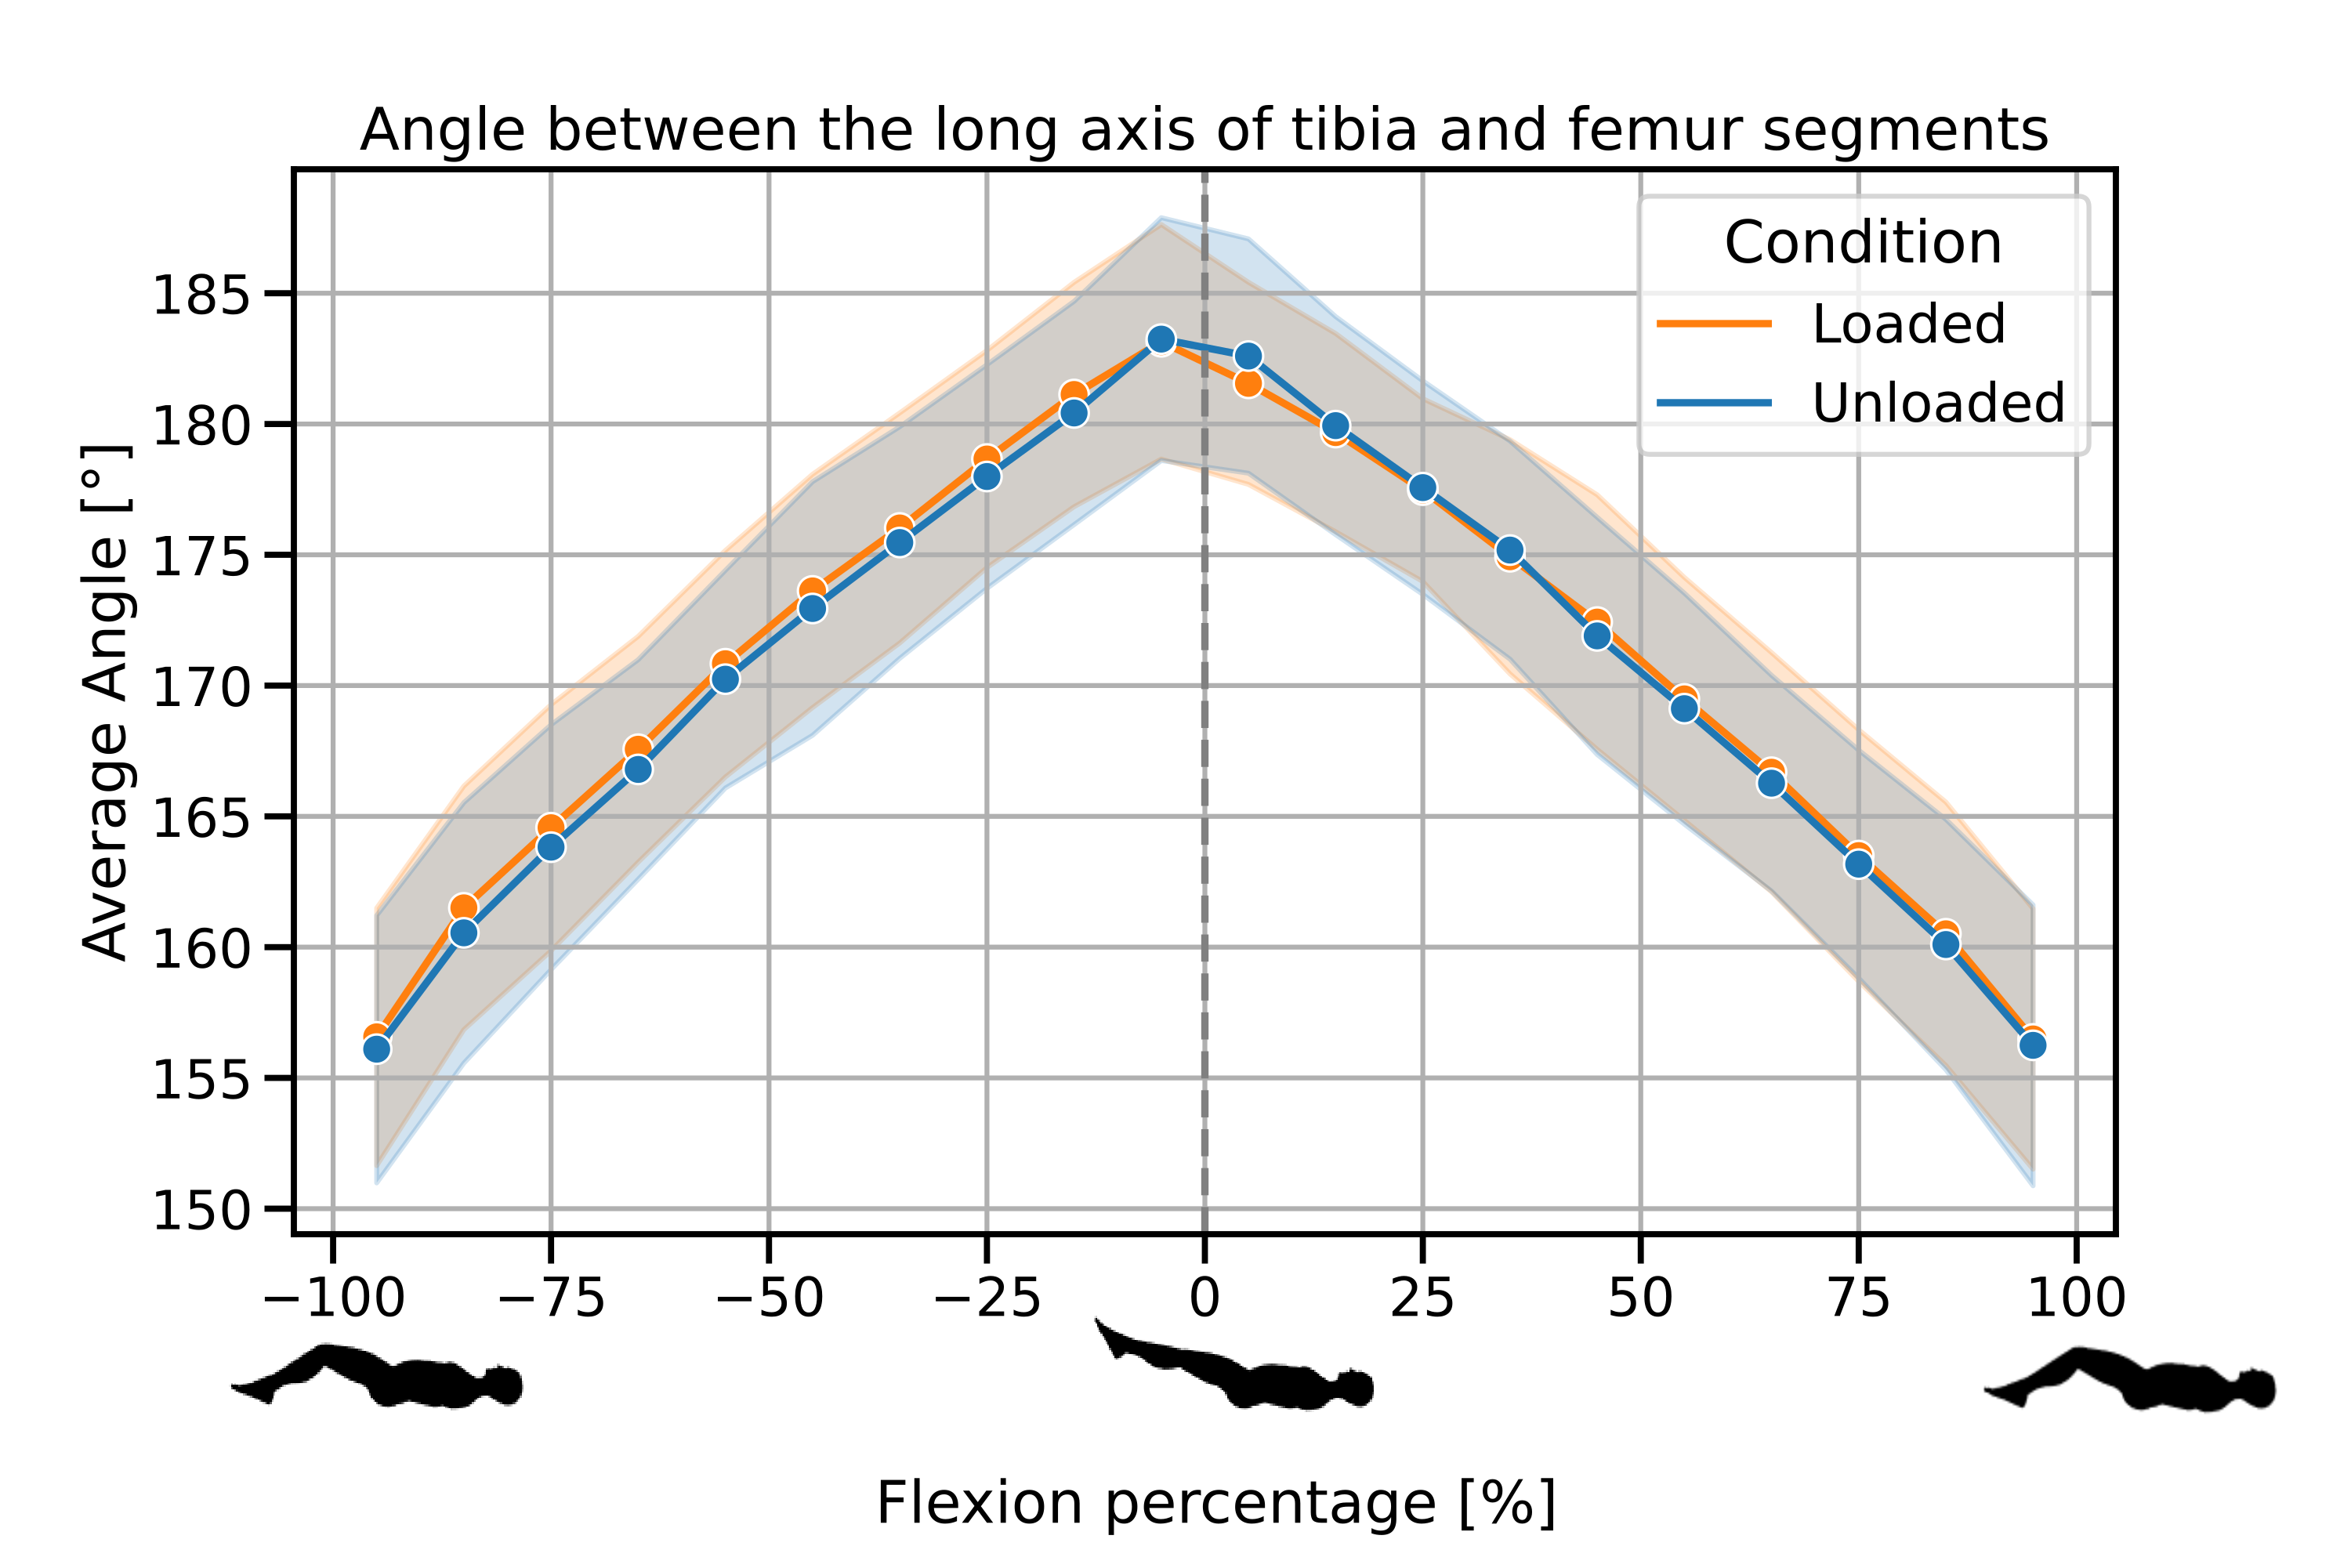
\includegraphics[width=0.7\linewidth]{angle_no_13_stick}
	\caption{Average angle between the long axes of the bone segments with respect to time during the motion cycle under loaded and unloaded condition.The x-axis ticks represent the centers of bins, each with a width of 10 percentage units. The shaded regions represent one standard deviation uncertainty across all the datasets. Angles greater than 180° imply hyperextension. Both loaded and unloaded conditions exhibit a similar pattern: : the angle increases as the knee extends, peaking slightly beyond 180° at maximum extension, before decreasing symmetrically as the motion approaches 100\% flexion}
	\label{fig:anglegraphstickman}
\end{figure}

No significant differences were observed between the loaded and unloaded conditions for any of the bins, as given in table \ref{tab:p_values_combined}. 

\textbf{Distance calculation }

The Euclidean distance between two points on the tibia and femur segments was measured throughout the flexion-extension cycle for both loaded and unloaded conditions. The aggregated results are shown in Figure \ref{fig:resultsdistancestickman}
\begin{figure}[H]
	\centering
	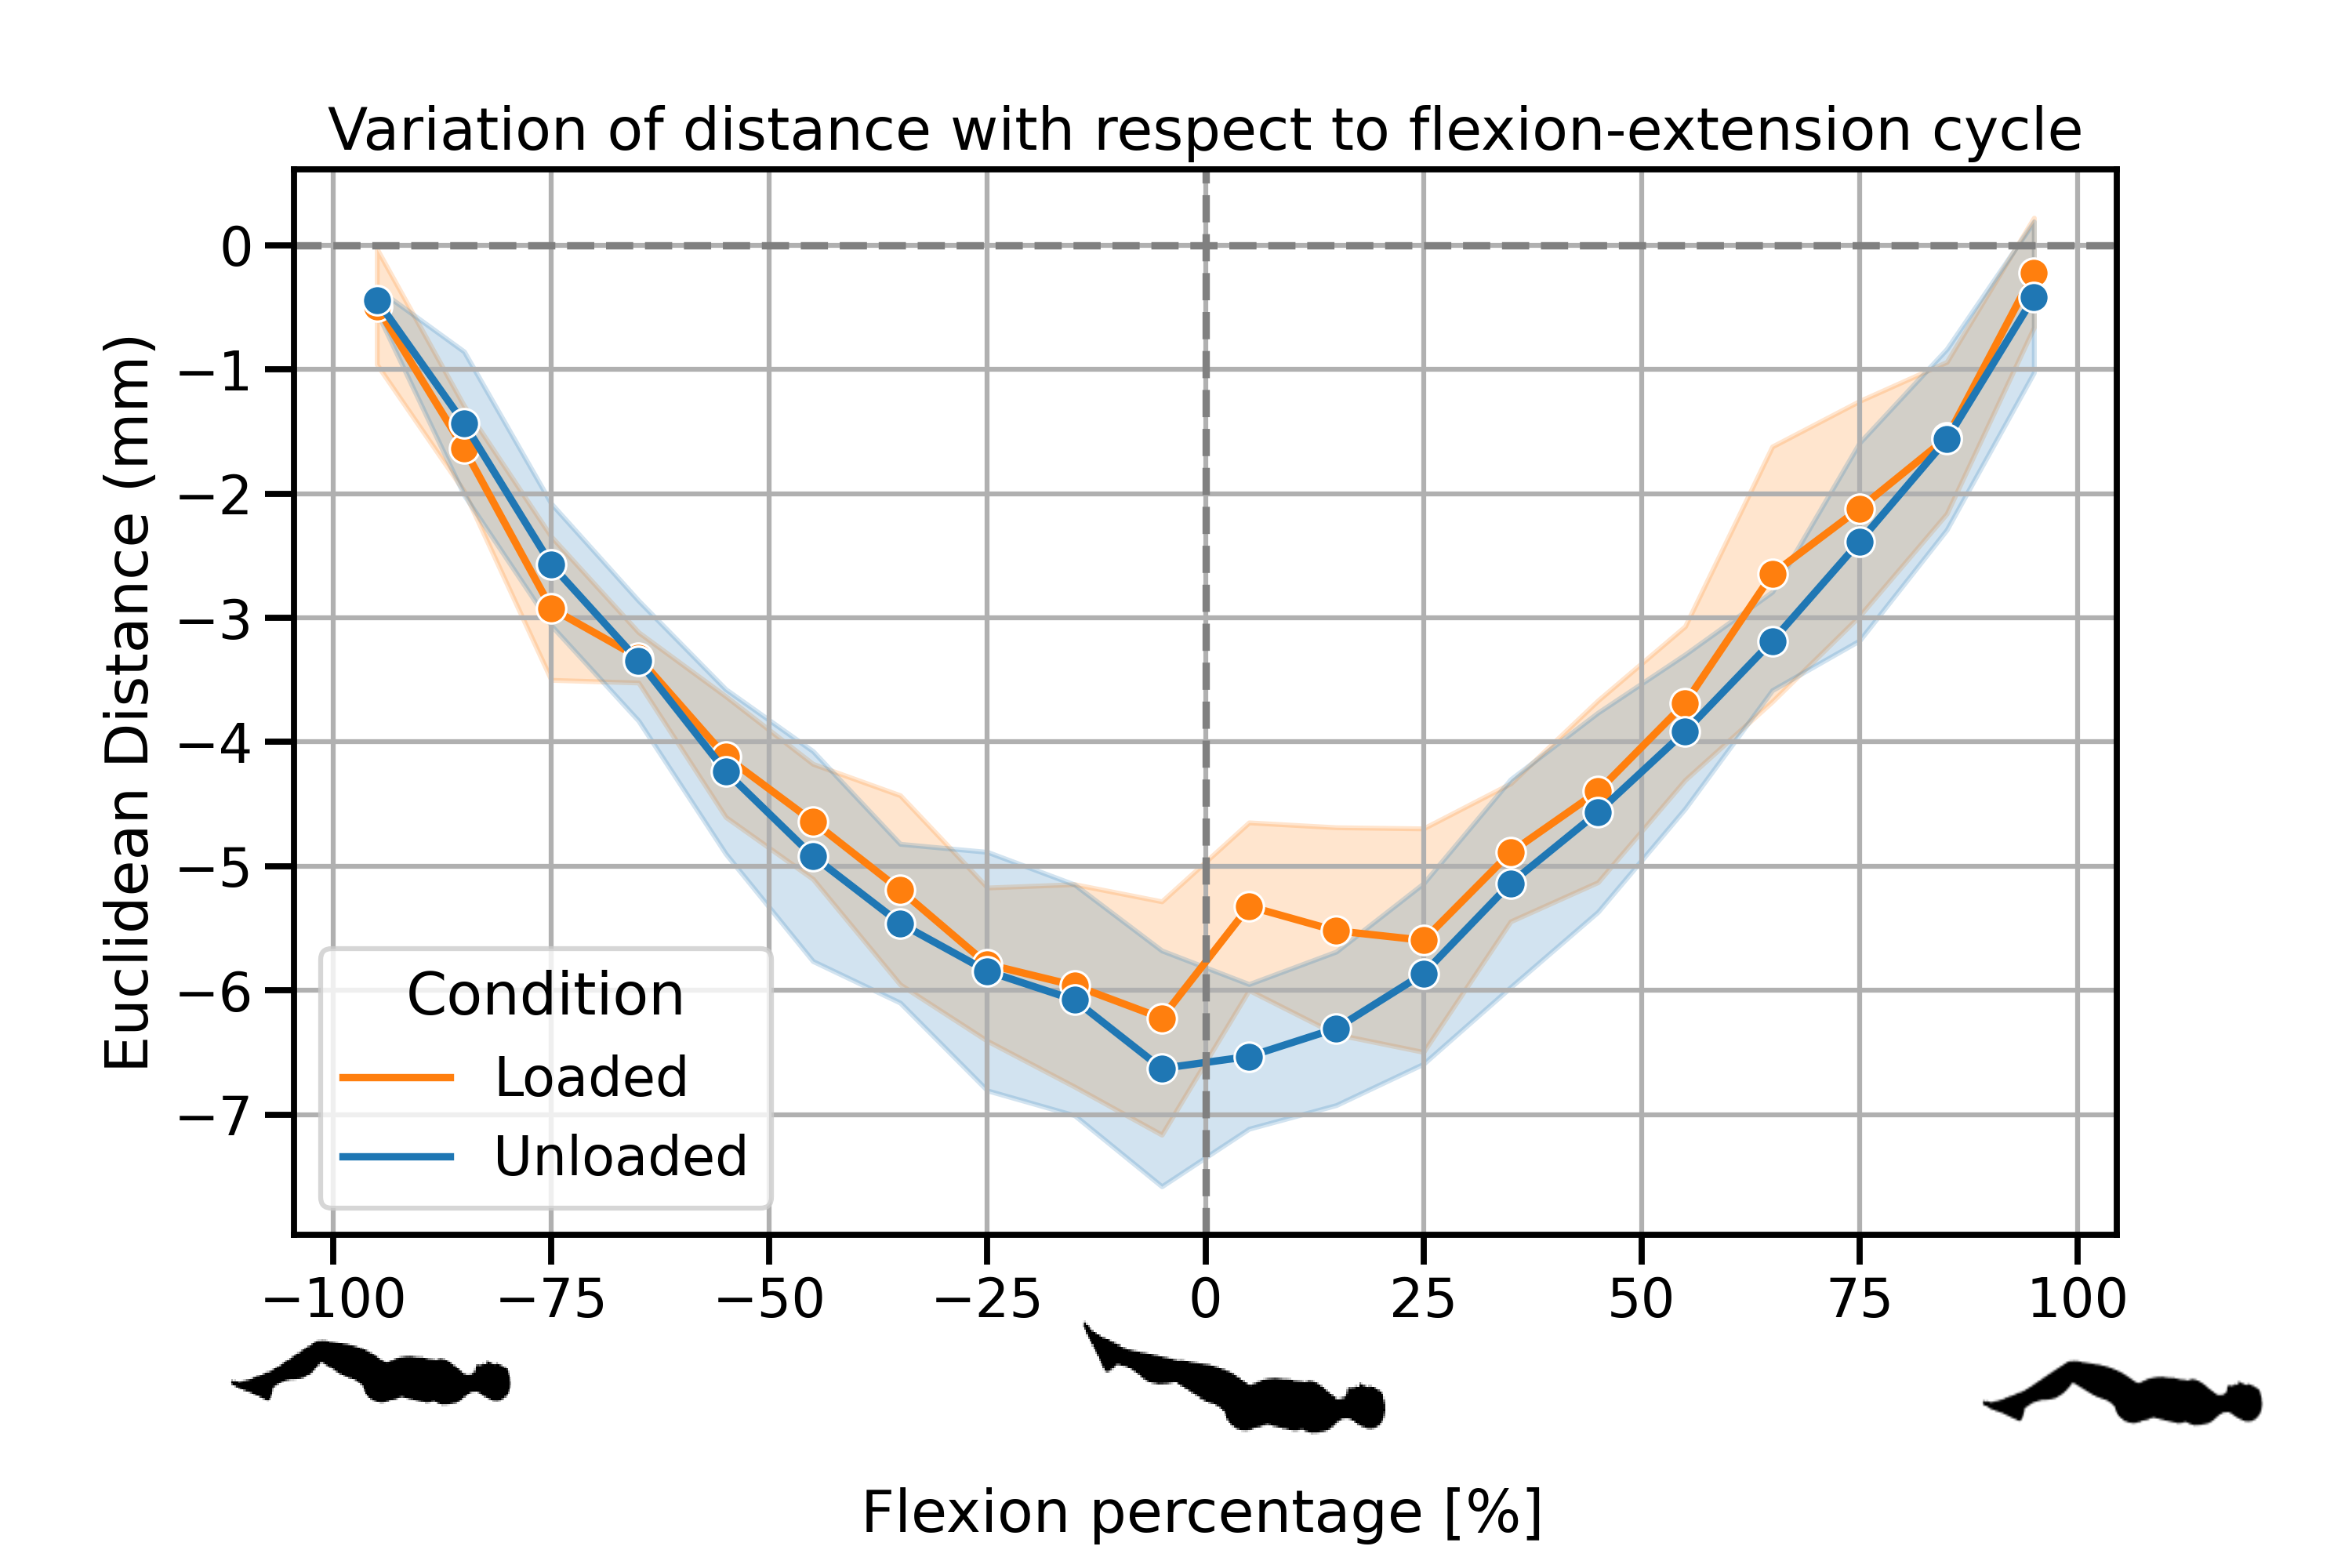
\includegraphics[width=0.7\linewidth]{distance_no_13_stick}
	\caption{Plot showing the variation of euclidean distance between the anatomical landmarks on the femur and tibia with respect to time in the motion cycle. All distances are relative to the baseline measurement at -100\% flexion, set at 0 mm. The shaded region represents one standard deviation uncertainty across all datasets for each condition. In both loaded and unloaded conditions, the distance decreases during the extension half of the cycle, indicating that the segments are coming closer together, and then increases during the flexion half, suggesting the segments are moving further apart.}
	\label{fig:resultsdistancestickman}
\end{figure}

The null hypothesis was rejected for only the movement range between 0-10\% flexion. No significant differences were observed for the remaining bins, as noted in table \ref{tab:p_values_combined}. 
\begin{table}[H]
	\centering
	\caption{Comparison of P-Values Across Flexion Percentage Ranges for Different Measurements}
	\label{tab:p_values_combined}
	\begin{tabular}{@{}ccc@{}}
		\toprule
		Flexion Percentage Range & p-value (Distance) & p-value (Angle) \\ \midrule
		-100\% to -90\% & 0.809 & 0.885 \\
		-90\% to -80\% & 0.518 & 0.762 \\
		-80\% to -70\% & 0.329 & 0.808 \\
		-70\% to -60\% & 0.914 & 0.781 \\
		-60\% to -50\% & 0.753 & 0.831 \\
		-50\% to -40\% & 0.535 & 0.825 \\
		-40\% to -30\% & 0.562 & 0.847 \\
		-30\% to -20\% & 0.915 & 0.808 \\
		-20\% to -10\% & 0.838 & 0.801 \\
		-10\% to 0\% & 0.516 & 0.973 \\
		0\% to 10\% & \textbf{0.016} & 0.703 \\
		10\% to 20\% & 0.129 & 0.918 \\
		20\% to 30\% & 0.617 & 0.969 \\
		30\% to 40\% & 0.595 & 0.928 \\
		40\% to 50\% & 0.737 & 0.863 \\
		50\% to 60\% & 0.576 & 0.899 \\
		60\% to 70\% & 0.305 & 0.883 \\
		70\% to 80\% & 0.626 & 0.913 \\
		80\% to 90\% & 0.977 & 0.898 \\
		90\% to 100\% & 0.574 & 0.942 \\
		\bottomrule
	\end{tabular}
	\begin{minipage}[t]{\linewidth} % Adjusting the width if necessary
		\bigskip
		\textbf{Note:} This table presents the p-values obtained from independent t-tests comparing the mean Euclidean distances and angles between loaded and unloaded conditions across predefined flexion percentage ranges. Each range represents an interval of 10\% in the flexion-extension cycle, with averages taken across all datasets. Significant p-values (p \textless 0.05) are highlighted in bold.
	\end{minipage}
\end{table}
\section{Discussion}

The accuracy and reliability of the measurements obtained from the dynamic MRI scans are influenced by several factors that need to be considered to ensure meaningful results. One significant factor is the overall bulk movement of the leg during the scan. If the femur is not properly fixated, the entire leg might shift, leading to inaccurate measurements. Ensuring that the thigh is securely positioned on the device with the thigh strap is critical for minimizing this movement. Additionally, improper fixation can allow the upper leg to lift or shift laterally, further compromising the accuracy of the measurements. This overall instability can be exacerbated by the entire leg shifting longitudinally within the scanner, causing misalignment and poor-quality output.

Another important factor is muscle exhaustion. At the start of the exercise, volunteers might overexert themselves, leading to fatigue as the exercise progresses. This can cause variations in the range of motion and affect the position of the leg, resulting in inconsistent data. While the controlled exercise pace, guided by a metronome, aims to standardize the movement, individual differences in endurance can still introduce variability.

With these considerations in mind, the following sections discuss the specific results of edge tracking and segmentation, angle measurement, and distance calculation in detail.

\subsection{Edge tracking and segmentation}
The accuracy of segmentation in this study is fundamentally tied to the precision of the introduced edge tracking, as the segment boundary is defined by the detected edges. A significant factor that compromises edge tracking accuracy is through-plane motion of the bones, leading to inaccurate transformations. The algorithm is specifically designed to manage only rigid transformations within a single plane; therefore, any deviations introduced by through-plane motion significantly impair edge detection and, consequently, segmentation accuracy.

Through-plane motion is particularly problematic for the tibia compared to the femur, primarily due it having more degrees of freedom, as illustrated in Figure \ref{fig:sixdegrees}, which details the six degrees of freedom of the tibia's movement relative to the femur. Despite the lower leg being secured at the ankle with Velcro straps and the knee cradled in a wedge positioner to limit movement predominantly to one plane, complete immobilization is not achievable. This limitation is especially pronounced in subjects with smaller bones, where even additional padding at the wedge positioner was insufficient to prevent all undesired motion. While localizers are employed prior to the scans in both extended and flexed positions to ensure that the slice moves only within a predetermined single plane, certain rotations cannot be fully corrected by simply angling the localizer and may still be evident in the final images. 
Figure \ref{fig:edgebad} showcases this problem faced by the edge tracking algorithm: 

\begin{figure}[H]
	\centering
	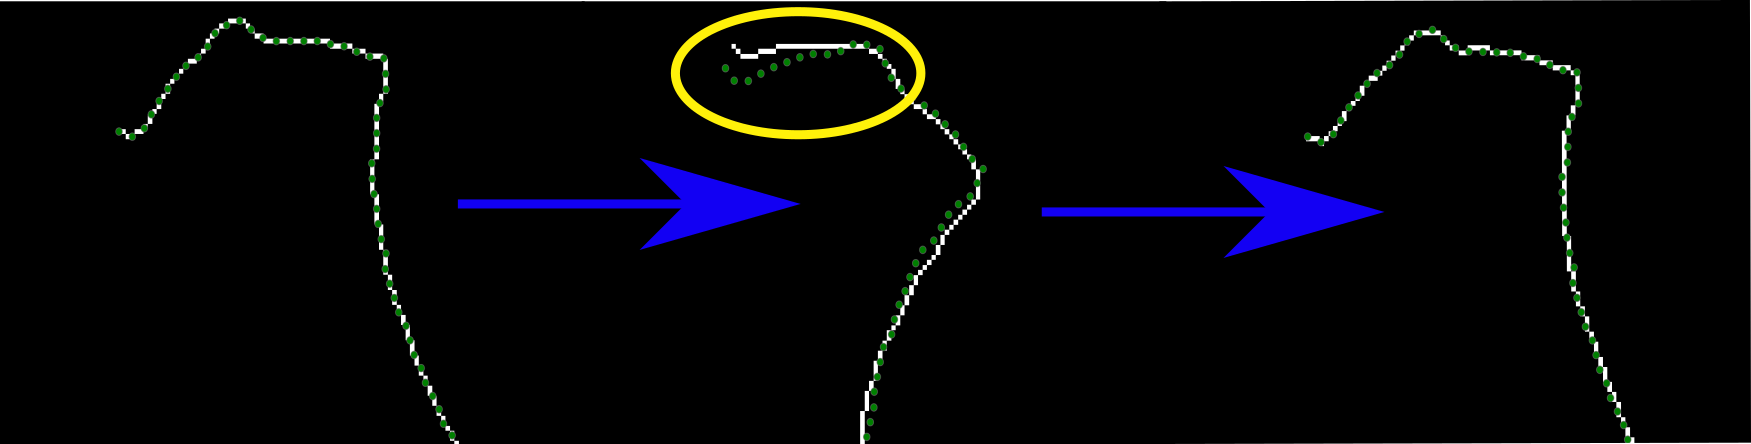
\includegraphics[width=0.9\linewidth]{three_try2}
	\caption{Three frames at -100\%, 0\%, and 100\% flexion are displayed, showcasing the binary edge of the tibia boundary (in white) alongside reference coordinates (in blue) during the edge tracking process. The images reveal that the algorithm struggles to accurately track the transformation between subsequent frames, especially evident in the misalignment of blue points near the proximal tibia in the middle frame (highlighted with a yellow circle). However, alignment improves significantly in the final frame as the knee returns to its original position. This variability is likely due to the leg's movement in and out of the scanning plane.}
	\label{fig:edgebad}
\end{figure}


Instances where significant deviations between transformed and target frames were observed like that shown above, led to the exclusion of the entire dataset from the analysis. This action was necessary because analyses based on misaligned data from any subject, whether during loaded or unloaded conditions, could result in misleading conclusions. Therefore, datasets were discarded to ensure the reliability and accuracy of the study's findings.

The datasets included in the analysis  demonstrated satisfactory segmentation. Edge tracking performance was consistently robust across both loaded and unloaded conditions as well as between different bones (femur and tibia). The similar trends in mean alignment errors for both conditions suggest that the edge tracking algorithm was equally effective regardless of the mechanical loading on the joints. Specifically, the mean alignment error for the femur in the unloaded condition was 0.331 mm ± 0.018 mm, compared to 0.37 mm ± 0.02 mm in the loaded condition. Similarly, for the tibia, the unloaded condition showed a mean alignment error of 0.32 mm ± 0.02 mm, while the loaded condition was slightly higher at 0.38 mm ± 0.02 mm. Additionally, the fact that even the datasets with the highest magnitude of mean alignment error (0.51 mm for the tibia under load) did not visually exhibit significant segmentation flaws reinforces the notion that the algorithm can tolerate a certain degree of error without compromising the overall quality of the segmentation.

To provide a context for these values, it is noted that similar metrics have been reported in MRI-based measurements. For example, Rathnayaka et al\,(2012) recorded an average alignment error per point of 0.23 mm in their study on the accuracy of MRI-generated 3D models of long bones \parencite{rathnayaka_quantification_2012}. 


\subsection{Angle calculation}

The change in the angle between the long axes of the bones at different points during the motion cycle is consistent with the expected biomechanics of the knee joint. The alignment of the femur and tibia is closest at full extension and diverges during flexion. The curve shape observed in Figure \ref{fig:anglegraphstickman} aligns with findings from similar studies \parencite{jeon_detection_2019}.

At full extension, the angles between the long axes of the bones are not perfectly parallel. This observation, likely influenced by the sagittal view used for measuring, aligns with findings from static scans where slight hyperextension is often reported \parencite{dai_comparing_2021}. 

\begin{figure}[H]
	\centering
	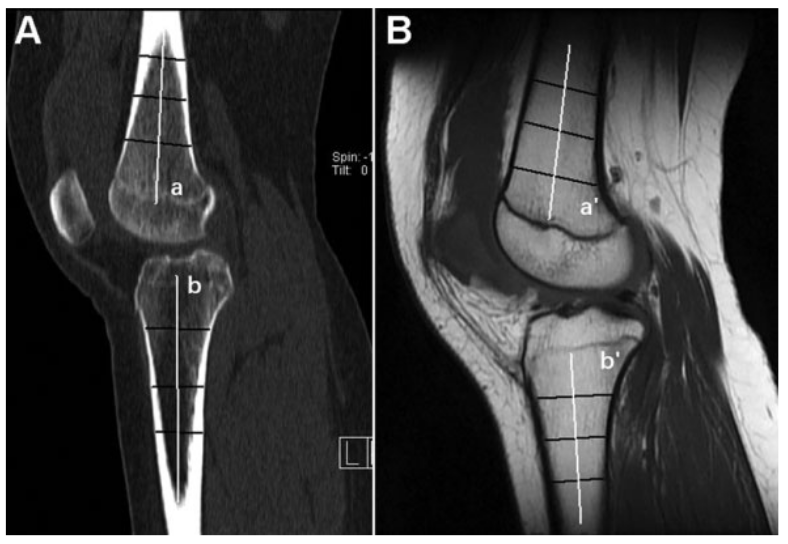
\includegraphics[width=0.7\linewidth]{dai_image}
	\caption{Femur (a) and tibia (b) shaft axes defined in static CT and T1-weighted MRI scans in the sagital view \parencite{dai_comparing_2021}. }
	\label{fig:daiimage}
\end{figure}

The null hypothesis was not rejected for any of the bins, as detailed in Table \ref{tab:p_values_combined}. This indicates that the method used in this study to calculate the angle was not affected by mechanical load.



\subsection{Distance calculation}

Figure \ref{fig:resultsdistancestickman} shows the variation in the Euclidean distance between anatomical landmarks on the femur and tibia throughout the extension-flexion cycle.

Significant differences were observed in the flexion percentage range between 0\% to 10\% with a P-value of 0.016. This would imply that external mechanical loading affects the spatial relationship between the femur and tibia, but only during the beginning of the flexion phase. 

This suggests that there is an underlying mechanism influencing the measured distance near terminal extension but not during other phases of motion. A likely candidate for this is the screw home mechanism (SHM) \parencite{kim_screw-home_2015}.The SHM involves the rotation of the tibia around the femur near terminal extension. It occurs due to the unequal lengths of the condyles. The medial femoral condyle is longer than the length of the lateral condyle, which causes the tibia to rotate externally in the last stages of extension.   This rotation occurs to lock the knee in a stable, fully extended position. Then, when flexion starts during the second half of the cycle, the tibia rotates internally, which 'unlocks' the knee for further flexion.

It has been previously reported that the impact of external loading increases the magnitude of internal rotation of the tibia relative to the femur \parencite{myers_vivo_2012}. Therefore, it seems that this internal rotation is more susceptible to changes in the distance between the defined anatomical landmarks due to external loading compared to external rotation. This susceptibility likely results in the significant differences observed during the initial phase of flexion, as the knee transitions from a fully extended, locked position to a flexed, unlocked state.  

Given these observations, it can be hypothesized that the response to external loading might serve as an indicator of SHM functionality. Notably, it has been demonstrated that SHM loss, characterized by reduced internal tibial rotation, occurs in patients with OA when compared to healthy controls, even without any applied external load \parencite{jeon_alteration_2020}. Additionally, quadriceps weakness has been identified as a significant risk factor for the development of OA \parencite{segal_is_2011}. This suggests that the external loading in this experimental setup, which induces quadriceps activation, could provide valuable diagnostic insights. Understanding the interaction between quadriceps strength and mechanical loading is crucial for detecting early signs of OA and developing targeted therapeutic strategies.

\section{Conclusion}

This study set out to explore the precision and practicality of a semi-automated segmentation process for analyzing dynamic MRI scans of the knee during flexion-extension cycles. The findings demonstrate the potential of this method to accurately track and quantify biomechanical parameters such as bone alignment and distances between anatomical landmarks under different loading conditions.

\textbf{Key Findings and Implications}

The metric used to quantify the accuracy of semi-automatic segmentation has been found comparable to those reported in the literature concerning MRI-based segmentation techniques. This semi-automated method is particularly advantageous for analyzing dynamic frames over time, making it highly suitable for clinical and research applications where advanced machine learning-based automatic segmentation techniques are not yet available for dynamic CINE images. The approach facilitates rapid and efficient analysis of a large number of frames and requires minimal computational power. Moreover, once the bones are segmented, a wide range of biomechanical analyses can be conducted, providing comprehensive insights into joint mechanics, beyond those attempted in this study.

The analysis of the angle between the long axes of the tibia and femur showed no significant differences between loaded and unloaded conditions. Any deviation from this trend while measuring patients with underlying conditions with OA could indicate potential pathological issues.

The distance measurement between anatomical landmarks on the tibia and femur revealed significant differences between loaded and unloaded condition during the early phase of the flexion. This variation can be attributed to the screw-home mechanism, emphasizing the sensitivity of the knee joint's biomechanics to external loading. These findings underscore the importance of considering external loading in biomechanical analyses and suggest that the method could be a valuable tool for potential diagnosis and research.



\textbf{Limitations and Future Work}

Despite its promising results, this study's methodology is limited by its reliance on a single 2D slice. This approach overlooks the tibia's six degrees of freedom relative to the femur, potentially omitting critical aspects of knee kinematics. Future work should aim to extend this methodology to 3D, which would not only address current method's issues in edge tracking, but also allow for a complete assessment of knee joint kinematics, providing a more holistic understanding of its movements and interactions.

Additionally, the semi-automated segmentation method demonstrated here can be adapted to analyze patellofemoral kinematics. The patella shows well-defined edges in the images, making it a suitable candidate for this processing pipeline. Given the patella's significant role in knee mechanics \parencite{powers_evidence-based_2017}, this extension would provide valuable insights and complement the current analysis of tibiofemoral interactions.

In conclusion, the semi-automated segmentation process evaluated in this study offers a robust and efficient method for analyzing dynamic MRI scans of the knee. By enabling accurate tracking of biomechanical parameters and accommodating various analyses, it presents a valuable tool for both clinical diagnostics and biomechanical research. While current limitations highlight the need for 3D analysis to fully capture knee kinematics, the potential applications of this method are vast, paving the way for more comprehensive and insightful studies of knee joint mechanics.
% ----------------------------------------------------------------------------
% Bibliography
% ----------------------------------------------------------------------------
\cleardoublepage
\phantomsection
\addcontentsline{toc}{section}{\refname} % to add Bibliography to toc
\printbibliography

% --------------------------
%\cleardoublepage
%\begin{appendix}
%\section{Appendix}
%%
%%The non aggregated results for Figures \ref{fig:anglegraphstickman} and \ref{fig:resultsdistancestickman} are shown below: 
%%\begin{figure}[H]
%%	\centering
%%	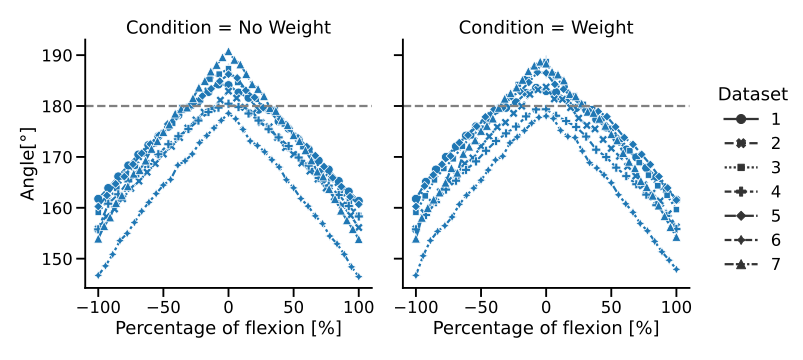
\includegraphics[scale=0.42]{angle_non_agg}
%%	\caption{Non aggregated results for the angle between the long axis of the bone segments. Loaded and unloaded measurements are shown in their respective columns.}
%%	\label{fig:anglenonagg}
%%\end{figure}
%%
%%\begin{figure}[H]
%%	\centering
%%	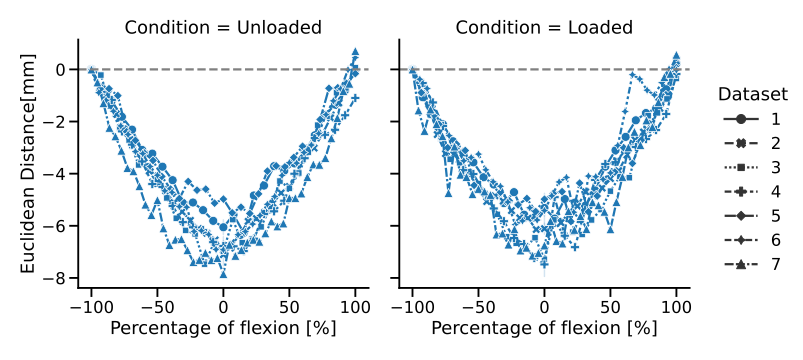
\includegraphics[scale=0.42]{norm_non_agg}
%%	\caption{Non aggregated results for the euclidean distance between anatomical landmarks on the femur and tibia. Loaded and Unloaded conditions are shown in their respective columns.}
%%	\label{fig:normnonagg}
%%\end{figure}
%
%
%
%
%\end{appendix}

% ----------------------------------------------------------------------------
% Statutory declaration
% ----------------------------------------------------------------------------
\makeThesisDeclaration

\end{document}

